\documentclass[a4paper,11pt,oneside,%twoside to print on the back of pages
headsepline,												% Linie für Kopfzeile
footsepline,												% Linie für Fußzeile
bibtotocnumbered									% numb point literaturverz in inhaltsverz => bibliography=tot ocnumbered
]{scrreprt}
%----------------------------------------------------------------------------------------------------------------------------------------------
% STANDART LIBS
\usepackage[T1]{fontenc}
\usepackage[utf8]{inputenc}
\usepackage[ngerman]{babel}    % Deutsche Sprache in automatisch generiertem

% DRUCKBEREICH: \areaset[BCOR]{textwidth}{textheight} %TODO understand
% BCOR ist "Binding Correction", also wieviel Innenrand verloren geht
% A4 hat 297mm x 210mm
% wenn keine Marginalien, dann ist Breite 15cm vielleicht besser
\areaset[1.5cm]{14cm}{25cm} 
%% Die folgende Zeile sorgt dafür, daß die Fußnoten eingerückt werden,
%% und zwar um 2em (class scrbook).
\deffootnote{2em}{2em}{\textsuperscript{\normalfont\thefootnotemark} }

%----------------------------------------------------------------------------------------------------------------------------------------------
% ADDITIONAL LIBS

\usepackage{grffile} %remove file names of images

% Wrapping text around figures
\usepackage{wrapfig}  %
% containers for things that cannot be broken over a page -> example table, figure
\usepackage{float}
% provides many ways to customise the captions in floating environments
\usepackage{caption} % http://www.ctex.org/documents/packages/float/caption.pdf
% same for subfigues
\usepackage{subcaption} % hint include subpicture

%% Unterstützung für Graphiken und Farben
\usepackage[pdftex]{graphicx}
%\usepackage[pdftex]{color}
%\definecolor{DSblue}{rgb}{0,0,0.9}   % example defining a color



% INDEX/GLOSSARY %TODO
%Defines commands for use with MakeIndex
%\usepackage{makeidx} % -> en.wikibooks.org/wiki/LaTeX/Indexing pctex.com/files/managed/3/3a/makeindx.pdf
%\usepackage[xindy,toc]{glossaries}
\usepackage{acronym} %Abkürzungsverzeichniss

%BIBTEX
%used by biblatex for qutes
\usepackage[babel,german=quotes]{csquotes} % load after inputenc
% cite package -> 1. pdflatex xx.tex 2. biber xx 3. pdflatex xx.tex
\usepackage[style=authoryear,backend=biber]{biblatex} %TODO check diff cite styles
% loads the bib file
\addbibresource{bachelorBib.bib}


% cross referencing and hyperrefs
\usepackage[                % FIXME explain
   pdftex,                  % Ausgabe-Medium: PDF
   colorlinks=true,         % farbige Links in der Bildschirm-Version?
   pdfstartview=Fit,       % wie soll Acrobat starten?
   linkcolor=black,         % Farbe für Querverweise
   citecolor=black,         % Farbe für Zitierungen
   urlcolor=black,          % Farbe für Links
   bookmarks=true
   ]{hyperref}
% non clickable URL   		
\usepackage{url} %TODO remove if hyperref is better

% TODONOTES -> http://tex.stackexchange.com/questions/9796/how-to-add-todo-notes
\usepackage{lipsum}                     % Dummytext
\usepackage{xargs}                      % Use more than one optional parameter in a new commands
\usepackage[pdftex,dvipsnames]{xcolor}  % Coloured text etc.
% -> www.tex.ac.uk/ctan/macros/latex/contrib/todonotes/todonotes.pdf
\usepackage[colorinlistoftodos,prependcaption,textsize=tiny]{todonotes}
\newcommandx{\unsure}[2][1=]{\todo[linecolor=red,backgroundcolor=red!25,bordercolor=red,#1]{#2}}
\newcommandx{\change}[2][1=]{\todo[linecolor=blue,backgroundcolor=blue!25,bordercolor=blue,#1]{#2}}
\newcommandx{\info}[2][1=]{\todo[linecolor=OliveGreen,backgroundcolor=OliveGreen!25,bordercolor=OliveGreen,#1]{#2}}
\newcommandx{\improvement}[2][1=]{\todo[linecolor=Plum,backgroundcolor=Plum!25,bordercolor=Plum,#1]{#2}}
\newcommandx{\thiswillnotshow}[2][1=]{\todo[disable,#1]{#2}}

% Print graphics
% tikz print graphs: http://www.texample.net/tikz/examples/
% bytefield – Create illustrations for network protocol specifications

% source code include
\usepackage{listings} % -> %TODO use minted
\usepackage{minted}

\makeatletter
\newcommand*{\rom}[1]{\expandafter\@slowromancap\romannumeral #1@}
\makeatother

%----------------------------------------------------------------------------------------------------------------------------------------------
% ADDITIONAL LIBS TO CHECK

%linien in Tabellen
\usepackage{booktabs}
\usepackage{anysize}
\usepackage[onehalfspacing]{setspace}


% math for matrix and $$
%\usepackage{amsmath}
%\usepackage{amssymb}

%\usepackage{lmodern}

%\usepackage{multido}    % FIXME ???????????
%\usepackage{everysel}   % FIXME ???????????
 
%% besserer Flattersatz: \RaggedRight
\usepackage{ragged2e}

% from exposee
\usepackage{latexsym}         % Fuer recht seltene Zeichen

\usepackage[a4paper,lmargin={2.5cm},rmargin={2.5cm},tmargin={3cm},bmargin={2.5cm}]{geometry}
\usepackage{enumerate}

\newcommand{\HRule}{\rule{\linewidth}{0.5mm}}

\pdfinfo{
	/Title		(Synchronisation von Binärbaum-indexierten, verteilten InMemory-NoSQL-Datenbanken)
	/Subject		(Bachelorarbeit)
	/Author		(Paul Kitt)
}
%----------------------------------------------------------------------------------------------------------------------------------------------
\pagenumbering{roman}
\begin{document}

%TODO set 1,5 zeilenabstand , verdana, schriftgroesse 10
%TODO check bewilligten title 


\begin{titlepage}
	\begin{center}
		\begin{figure}[!htb]
			\minipage{0.5\textwidth}
				\begin{center}
			  		
\includegraphics[width=0.5\textwidth]{bilder/htwLogo.jpeg}
				\end{center}
			\endminipage\hfill
		 	\minipage{0.5\textwidth}
				\begin{center}
			 		
\includegraphics[width=0.5\textwidth]{bilder/Spinning_O_Wheel-200.png}
				\end{center}	
			\endminipage
		\end{figure}
	
		 \vfill
		 \HRule \\[0.4cm]
	    {\bfseries\Large
	        \begin{LARGE}
	        Synchronisation von Binärbaum-indexierten, verteilten
			InMemory-NoSQL-Datenbanken\\
	        \end{LARGE} 
	    }    
		\HRule \\[1.5cm]
			\begin{minipage}{1.0\textwidth}
				\begin{flushleft}
				\Large	Abschlussarbeit
				\end{flushleft}
			\end{minipage}
			\vfill
			\begin{minipage}{1.0\textwidth}
				\begin{flushleft}
					\Large zur Erlangung des akademischen Grades\\
					\Large Bachelor of Science (B.Sc.)
				\end{flushleft}
			\end{minipage}
			\vfill
			\begin{minipage}{1.0\textwidth}
				\begin{flushleft}
					\Large an der
				\end{flushleft}
			\end{minipage}
			\vfill
			\begin{minipage}{1.0\textwidth}
				\begin{flushleft}
					\Large Hochschule für Technik und Wirtschaft Berlin\\
					\Large Fachbereich Wirtschaftswissenschaften \rom{2}\\
					\Large Studiengang Angewandte Informatik\\
				\end{flushleft}
			\end{minipage}
			\vfill
			\begin{minipage}{1.0\textwidth}
				\begin{flushleft}
					\Large 1. Prüfer: Prof. Dr.-Ing. Hendrik Gärtner\\
					\Large 2. Prüfer: Jens-Peter Haack\\ \todo[inline]{Titel Adademischer Grad}
				\end{flushleft}
			\end{minipage}
			\vfill
			\begin{minipage}{1.0\textwidth}
				\begin{flushleft}
					\Large Eingereicht von Paul Kitt
				\end{flushleft}
			\end{minipage}

		\vfill
		\begin{minipage}{1.0\textwidth}
			\begin{flushleft}
				{\Large \today}
			\end{flushleft}
		\end{minipage}
		\vfill

	\end{center}
\end{titlepage}
\tableofcontents
\newpage
%\todo[inline]{table of table}
%\todo[inline]{table of listings}
Abkürzungsverzeichniss:\\
\begin{acronym}[EB-Baum] % option laengest abk def einzuglänge
 	\acro{EB-Baum}{Elastische Binär Baum}
 	\acrodefplural{EB-Baum}[EB-Bäume]{Elastische Binär Bäume}
 	\acro{ID}{Identifikationsnummer}
\end{acronym}
\renewcommand\listoflistingscaption{Verzeichnis aller Codebeispiele}
\listoflistings

	%---------------------------------------------------------------------------------------------------------------------------------------------------	
\chapter{Einleitung}
\pagenumbering{arabic}
\todo[inline]{Hintergrund, größerer Rahmen, kurze Aufgabenstellung}
 		\begin{enumerate}[1.]
			\item  Problemstellung und Motivation
			\item Zielsetzung
			\item Rahmen und Aufbau der Arbeit
		\end{enumerate}
		
	Mögliche Punkte:
	-> Motivation
	-> Aufgabenbeschreibung
	-> Inhalt und Aufbau der Arbeit	
		
	%---------------------------------------------------------------------------------------------------------------------------------------------------	
\chapter{Grundlagen}
\todo[inline]{	theoretische Grundlagen, Beschreibung von Systemen(nur insoweit, als das diese Grundlagen und Beschreibungen unbedingt für das Verständnis erforderlich sind und nicht als bei studierten Informatikern vorausgesetzt werden kann)}

	\begin{enumerate}[1.]
			\item Grundlagen verwendeter Algorithmen
				\begin{enumerate}[1.]
					\item Binär Bäume
					\item Elastische Binär Bäume
				\end{enumerate}
			\item Definition von Begriffen
				\begin{enumerate}[1.]
					\item Verteilung
					\item Synchronisation
					\item NoSql -> CAP, ACID theoreme die meine db erfüllt 
				\end{enumerate}
			\item Grundlagen Datenbanken (Verteilung, Synchronisation)
				\begin{enumerate}[1.]
					\item MySql
					\item NoSql 
					\item Baumbasierter Indexe
				\end{enumerate}
	\end{enumerate}

\section{Elastische Binär Bäume}
\label{sec:ebTreeGrundlagen}
%TODO kurzedef binaer baum std werke
Bei den \enquote{Elastischen Binär Bäumen} handelt es sich um speziell optimierte Variante der \enquote{Binären Suchbäume}. Entwickelt wurden das Konzept von Willy Tarreau\autocite{Tarreau} im Rahmen einer Forschung zum Thema \enquote{Event-scheduling for user-space network applications} und eignen sich daher auch speziell für Betriebssystem Scheduler, bei welchen schnelles priorisieren nach Zeit oder Dringlichkeit wichtig ist. Daten die mit Binär- oder Ganzahlen, wie Integer oder Long, indexiert sind können in dieser wenig bekannten Datenstruktur sehr effizient verwaltet werden. Dabei ist der \enquote{\ac{EB-Baum}} sehr performant wenn es zu sehr vielen den, Baum verändernden, Operationen, wie: Einfügen, Ändern, Abfragen oder Löschen kommt.\unsure{wie richtig zitieren?}\\
Einfügeoperationen und das Abfragen von Blättern wird in O(log n) bewältigt. Löschen in O(1).\\

Als Ausgangskonzepte dienten bei seiner Entwicklung der \enquote{balanciertem Binär Baum}\unsure{mention red black tree} und des \enquote{Radix Baumes}. Da aber Operationen wie Löschen von Blättern bei einem \enquote{balanciertem Binär Baum} O(log n) kosten und der Baum aber gerade Operationen wie diese möglichst schnell bewältigen soll ein signifikanter Nachteil. Bei den \enquote{Radix Bäumen}, die sich laut dem Entwickler Willy Tarreau\autocite[Absatz Introduction]{Tarreau} im Bezug auf Geschwindigkeit sehr gut eigenen, wird aber im Betrieb das allocieren von Speicher und die damit verbundene \enquote{Garbage Collection} zum Perfomanceproblem.\\

Daher ist der \ac{EB-Baum} eine hybride Form aus beiden um diese Mängel aus zu gleichen. Es handelt sich nicht um einen balancierten Baum, was in besonderen Fällen zu einer schlechteren Leistung als die eines \enquote{balanciertem Binär Baum} führt\unsure{mention example}. Die Blätter sind im Baum von links nach rechts aufsteigend, nach einer Binär- oder Ganzahl(e.g. Integer, Long) sortiert.\\

Eine weitere Besonderheit des \ac{EB-Baum} ist dass seine maximale Höhe durch den Datentyp der Schlüssel bestimmt wird.
So kann beispielsweise ein Baum dessen Schlüssel Werte des Datentypes \enquote{Long} sind maximal 64 Ebenen besitzen da der Datentyp aus 64 Bit besteht. Schlüssel werden durch die Abfolge ihrer Binären Repräsentation adressiert. Der Schlüssel dient hierbei wie eine Art binäre Karte. Begonnen am höchsten gesetzten Bits des Schlüssels und wird der Baum Knoten für Knoten durch laufen und an den Knoten bei einer Null links, bei einer Eins rechts abgebogen bis dass Blatt oder falls dieses nicht vorhanden das am naheliegendste gefunden ist

\subsection{Besonderheiten des Baumes}
Durch die besondere Beschaffenheit des Baumes lassen sich viele Operationen sehr leicht umsetzen wie:
\begin{itemize}
	\item \textbf{Abfragen}
	\begin{itemize}
		\item das Abfragen des ersten und letzten Schlüssels
		\item erlangen des nächst kleineren oder größerem Schlüssel zu einem gegeben Schlüssel
		\item genaues Finden eine Schlüssels
		\item das Finden des ähnlichsten Schlüssels falls dieser nicht enthalten ist
		\item einfaches Abfragen von Bereichen durch ein Prefix
		\item erlangen des vorherigem oder nächstem unterschiedlichen Schlüssel zu einem gegeben Schlüssel
		\item mehrfach auftretende Schlüssel werden immer in ihrer eingefügten Reihenfolge zurück gegeben
	\end{itemize}
	\item \textbf{Einfügen}
	\begin{itemize}
		\item Einfügen mit Duplikaten: Falls ein Werte bereits existiert wird ein Duplikat angelegt
		\item Einfügen von nur einzigartigen Schlüsseln: Falls der Schlüssel vorhanden wird Existierende zurück gegeben
	\end{itemize}
\end{itemize}


\subsection{Aufbau des Baumes}
In dem originalem von Willy Tarreau verfassten Konzept\autocite[Absatz Definitions]{Tarreau} werden die Daten, die Baum hält, in \enquote{EB Knoten}
gespeichert. \enquote{EB Knoten} bestehen aus zwei Teilen:
\begin{itemize}
\item Knoten: verknüpft Blätter sowie anderen Knoten
\item Blatt: ist durch einen Schlüssel adressiert, hält Daten e.g. Referenz auf ein Datenobjekt
\end{itemize}


\begin{wrapfigure}{r}{0.6\textwidth}
  \begin{center}
    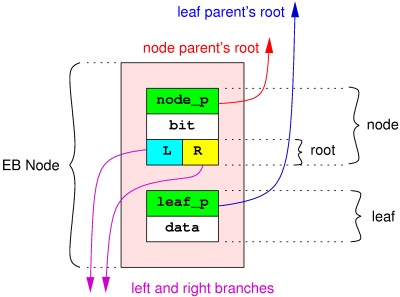
\includegraphics[width=.6\linewidth]{bilder/Ebnode.png}
  \end{center}
 \caption{EB-Knotenelement}
\end{wrapfigure}
Die Aufgabe eines Blattes ist sehr simpel. Es dient nur dazu eingefügte Daten durch einen Pointer zuhalten. Dabei ist es mit einem Schlüssel adressiert und besitzt eine Referenz auf seinen Elternknoten, sowie auf seinen EB-Ursprungsknoten\unsure{SPW fragen}.\\

Ein jedes Knotenelement besteht aus einer Referenz auf sein höher liegenden Elternknoten, dem Ebenenbit \unsure{Darf ich das Bild benutzen?} und zwei Referenzen auf seine Kinderknoten. \\ Das Ebenenbit ist eine Zahl und repräsentiert binär die niedrigste Bitposition des Schlüssels über dem alle Bits gleich sind. Alle unter dem Knoten liegenden Schlüssel haben sich somit bis zu diesem Bit die gleich Bitfolge. Der dritte Teil des Knotens ist die Wurzel die aus zwei Referenzen besteht zu entweder weiteren Knoten oder/sowie Blättern verweist. Da es sich um einen binären Baum handelt repräsentiert je Referenz das linke Bit 0 oder das rechte 1. Nur auf Ebene 0, mit dies repräsentierendem Ebenenbit, kann der Knoten zwei Blätter als Wurzel besitzen, da der Schlüssel sich nur um einen Wert an der letzten, nullten Bitstelle unterscheiden kann.\\
Auch wenn Knoten sich später verschieben können diese nie unterhalb des mit ihnen angefügtem Blattes oder in einen anderen Zweig des Baumes gelangen. Falls es erlaubt ist Duplikate einzufügen werden  Knoten mit negativen Ebenenbits versehen.\\

Eine weitere Besonderheit hier ist dass die Wurzelreferenzen nie unbelegt sind. Nur die Wurzel des Wurzelknoten des Baumes ist hier eine Ausnahme. Wenn seine zwei Wurzeln auf \enquote{null} referenziert ist der Baum leer. Sobald der Baum befüllt wird wächst dieser an seiner linken/\enquote{0-Wurzel}. Die rechte Wurzel referenziert immer auf \enquote{null}. Dadurch lässt sich der der Wurzelknoten einfach erkennen.
Sein Ebenenbit ist die höchste Ebene des Baumes und daher automatisch die binäre Länge des Schlüsseldatentyps, e.g. bei Schlüsseln des Datentyps Long ist das Ebenenbit 64.\\

\subsection{Einfügen von Daten}
Beim einfügen neuer Datensätze wird jeweils ein Blatt, das die Daten hält, sowie ein Knoten mit dem dass Blatt in Kombination eingefügt wird, eingefügt. Der einzige Fall in dem ein Blatt ohne Knoten angefügt wird ist wenn der Baum leer ist.

Beim Einfügen eines neuen Datensatzes wird ein gesamter \enquote{EB-Knoten} erstellt und an der richtigen Position eingefügt. Werden später weitere Werte gespeichert wird bei deren sortiertem einfügen der Baum umstrukturiert. Dies hat zur Folge dass Knoten und Blatt eines vorher übereinander liegenden \enquote{EB-Knoten} auseinander gezogen werden. Da sie aber noch durch gegenseitige Referenzen\unsure{logisch} verbunden bleiben wird der Baum als elastisch bezeichnet was zum Namen \enquote{\ac{EB-Baum}} führt.\\
Die enge Verknüpfung von Knoten und Blatt ist aber nicht zwingend notwendig. In einer, in Java implementierten, Umsetzung von Spinning Wheel, auf der später in dieser Arbeit eingegangen wird, wird ebenfalls beim Einfügen neuer Daten zu jedem Blatt ein Knoten erstellt aber später wenn der Baum sich verändert ist die Verbindung zwischen Knoten und Blatt nicht mehr nachvollziehbar.
\newpage
\section{NoSQL Datenbanken}
Das Idee der NoSQL Datenbanken ist anders als es erwarten lässt keine neue Erfindung. Schon die 1979 entwickelte \enquote{DBM} beruhte auf einem \enquote{Key/Hash} Konzept und auch in den 80er Jahren waren mit \enquote{Lotus Notes} und \enquote{Berkley DB} bereits Konkurrenz zu den bekannten SQL basierenden Datenbanken existent \autocite[1]{Edlich2010}. Daran dass immer mehr neue Datenbanken, die die ausgetreten Pfade der klassischen, relationalen Datenbanken verlassen, auf dem Markt erscheinen liegt viel mehr an den sich verändernden und rasant steigenden Anforderungen die heute an moderne Datenbanken gestellt werden. NoSQL ist nicht durch eine Organisation oder ein Gremium definiert worden sondern viel mehr Sammelbegriff einer neuen Generation von Datenbanken die dann unter dem Titel \enquote{NoSQL} zusammen gefasst wurden. Populäre Vertreter aus dieser Reihe sind z.B. Casandra, Redis, MongoDB und viele weitere. Eine Definition welche Anforderungen eine Datenbank erfüllen muss um in diese Kategorie zu fallen ist daher nicht klar definiert. In \enquote{NoSQL: EInstieg in die Welt nicht relationaler Datenbanken} nähert sich Prof. Stefan Edlich durch folgende Definitionen  einer generellen Beschreibung an. Unter NoSQL wird eine neue Generation von Datenbanksystemen verstanden, die meistens einige der folgenden Punkte berücksichtigen\autocite[2]{Edlich2010}:
\begin{itemize}
		\item Das zugrundeliegende Datenmodell ist nicht relational
		\item Die Systeme sind von Anfang an auf eine verteilte und horizontale Skalierbarkeit ausgerichtet
		\item Das System ist schemafrei oder hat nur schwächere Schemarestriktionen.
		\item Aufgrund der verteilten Architektur unterstützt das System eine einfache Datenreplikation
		\item Das System bietet eine einfache API
		\item Dem System liegt meistens auch ein anderes Konsistenzmodell zugrunde: Eventually Consistent und BASE, aber nicht ACID
\end{itemize}
Die Erweiterung eines bereits festgelegten Datenbankschemas, bei sich veränderten Anforderungen, kann bei relationalen Datenbanken zu problemen oder zu unerwünschten \enquote{Downtimes} führen. Daher werden Schemarestriktionen gelockert und ein einfaches sowie schnelle nachträgliches Ändern von Datenstrukturen ermöglicht. Durch Konzepte wie \enquote{Multiversion Cocurrency Control} kann die Datenstruktur im Hintergrund verändert und sobald der Vorgang abgeschlossen als neue Version in Betrieb genommen werden. Sie muss nicht gesperrt werden wie es beispielsweise einer komplexeren Änderung durch \enquote{ALTER TABLE} und damit verbundenen Anpassungen fordern würde.\\\\
Das Aufkommen von extrem großen Datenmengen in Bereichen von Terra bis im Extremfall Petabyte sind heute keine Seltenheit mehr sondern viel mehr Normalität. Die Entstehung vieler neuer NoSQL Datenbanken passierte zeitgleich mit der Entwicklung des Web 2.0 und diese deshalb für das Verwalten sehr großer Datenmengen ausgerichtet.
Dabei spielt die Möglichkeit wie einfach die Datenbank zu skalieren ist eine große Rolle. So müssen diese sowohl vertikal (scale up) als auch horizontal (scale out) Skalierbar sein. Die vertikale Skalierung wird durch ein einfaches verbessern der Datenbankhardware umgesetzt. Bei der horizontalen Skalierung wird die Masse an Daten und Last auf mehrere Instanzen aufgeteilt und ermöglicht eine Kosten günstigere und flexiblere Möglichkeit die Leistung des Systems zu erweitern. Dieser Prozess wird als \enquote{Sharding} bezeichnet
NoSQL Datenbanken sind nicht mehr wie viele relationale Datenbanken nur eine Datenbank sondern von sich aus bereits ein Datenbanksystem oder bieten einfache Möglichkeiten der Erweiterung zu diesem. Die Möglichkeit der Replikation steht dabei an zentraler Stelle, siehe \autoref{sec:VertDB}.\\\\
Je nach Anforderungen orientiert sich die Datenbanken an Modellen wie \enquote{ACID}\footnote{Atomicity, Consistency, Isolation, Durability} oder dem \enquote{CAP-Theorem} und lassen die Restriktionen relationaler Konkurrenten, die sich stark an \enquote{ACID} und dem Konzept der Transaktionen orientieren, hinter sich. So liegen die Ansprüche bei  Web 2.0 Anwendungen, wie z.B. Sociale Netzwerke, mehr auf schnellen Antworten, dem Halten immenser Datenmengen und Fehlertoleranz als auf Konsistenz und fehlerfreien Transaktionen.
Nichtsdestotrotz gibt es aber auch NoSQL Datenbanken die Transaktionen oder mindestens transaktionsähnliche Prozesse bieten um auch bereits bekannten Anforderungen zu genügen.

\subsection{Typen}
NoSQL Datenbanken lassen sich in vier Kategorien einteilen:
\begin{description}
   \item[Key/Value Stores] Daten werden in Schlüssel/Werte Paaren gespeichert. Dabei ist es oft möglich die Schlüssel in Namensräume zu sortiert und den Werten Datentypen zu zuweisen. Durch dieses einfache Schema lassen sich die Daten einfach aufteilen. Die Verarbeitung ist ebenso sehr schnell und effizient. Nachteil dabei ist dabei dass nur einfache Abfragemöglichkeiten verfügbar sind \autocite[131]{Edlich2010}. 
   \item[Wide Column Stores] Daten werden ähnlich den rel. Datenbanke in Tabellen gespeichert jedoch werden Werte gruppiert in Attribute spalten orientiert in jeweils eine eigene Tabelle geschrieben. Dies ermöglich ein einfaches Verarbeiten der Daten. Operationen wie jedoch Schreiben oder bestimmte Abfragen sind aufwendig.
   \item[Document Stores] Basiert auf dem Konzept strukturierte Daten in Dokumenten abzulegen. Auf diese wird mittels IDs referenziert und so ein Zusammenhang erstellt. Dateiformate sind dabei: JSON, YAML oder RDF.
   \item[Graphendatenbanken] Eignen sich besonders um den Zusammenhang zwischen Daten abbilden zu können. Die technischen Möglichkeiten immer komplexere Dinge wie Moleküle oder Linkstrukturen des  Internets zu erfassen steigern den Bedarf diese Daten in einem passendem Schema zu speichern. Die Daten werden dabei in Baum- oder Graphenstrukturen gespeichert.
\end{description}

\section{NoSQL relevante Konzepte}
\subsection{CAP-Theorem}
Das CAP-Theorem, auch als Brewer's Theorem bekannt, betrachtet drei Kriterien die an Datenbanken gestellt werden:
\begin{description}
\item[Konsitenz(Consistency)] Steht im CAP-Theorem dafür, dass die verteilte Daten-
bank nach Abschluss einer Transaktion einen konsistenten Zustand erreicht \autocite[31]{Edlich2010} und Veränderung auf allen Knoten erfolgt ist
\item[Verfügbarkeit(Avaibility)] bedeutet dass jede Anfrage die an einen nicht ausgefallenen Knoten gestellt wird beantwortet wird ganz gleich ob Erfolg oder Fehler \autocite[54]{Fowler2013}.
\item[Ausfalltoleranz(Partition Tolerance)] meint dass das System im Falle eines Ausfalls eines Knoten von Außen betrachtet noch Problemlos weiter funktioniert.
\end{description}
Je nach dem für welche Anforderungen die Datenbank ausgelegt es erfüllt sie Teile dieser drei Kriterien aber nie alle drei. 
\subsection{BASE-Konsistenzmodell}
Die Abkürzung BASE steht für Basically Available, Soft state, Eventual consistency. Der Ansatz des BASE-Konsistenzmodell verfolgt eine maximal hohen Verfügbarkeit und Leistung. Konsistenz wird dieser untergeordnet. Wo ACID einen pessimistischen Ansatz bei der
Konsistenz verfolgt, ist BASE ein optimistischer Ansatz, bei dem Konsistenz als ein Übergangsprozess zu sehen ist und kein fester Zustand nach einer Transaktion\autocite[33, 34]{Edlich2010}. Der Zustand von Konsistenz wird dabei am Ende auch erreicht aber erst irgendwann in einem bestimmten Zeitrahmen. Dieser neue Ansatz von Konsistenz wird als: Eventually Consistency bezeichnet. Dabei versteht sich BASE zu ACID nicht als sich gegenseitig ausschließend sondern, laut Eric Brewer \footnote{formulierte das CAP Theorem,Prof. an der UC Berkeley} eher als andere Seite eines Spektrums in dem relationale Datenbanken mehr zu ACID und NoSQL eher zu BASE tendieren.
\section{Verteilte Datenbankarchitekturen und Replikationsstrategien}
\label{sec:VertDB}
verteiltes system mit datenbanken %TODO std werke usen
Master slave
Multi Master
peer based
 
	%---------------------------------------------------------------------------------------------------------------------------------------------------	
\chapter{Anforderungsanalyse und Vorgehen}
\todo[inline]{	Bewertung von theoretischen Ansätzen, Konzepten, Methoden, Verfahren; informelle Aufgabenbeschreibung, klar formulierte Zielstellung  }
\begin{enumerate}[1.]
			\item Anwendungsumgebung
			\item Anforderungen und Szenarios
		\end{enumerate}
-> Vortrag

\section{Betriebliches Umfeld}
Diese von mir verfasst Arbeit entstand in enger Kooperation mit der neue entstehenden Spinning Wheel GmbH. Das hier implementierte und getestete Datenbankteilkonzept ist ein kleiner Bestandteil eines großen Softwareprojektes mit dessen Entwicklung die Firma sich beschäftigt. So wurde ich mit Idee und Grundkonzept beauftragt und bei deren Umsetzung von Herrn Jens-Peter Haack und Gernot Sänger bei theoretischen Fragen unterstützt.\\

Die Spinning Wheel GmbH befasst sich mit der Entwicklung neuer Softwarelösungen für das Backend von Mobilfunkinfrastruktur. Dabei steht das verarbeiten und speichern von Mobilfunksubscriberdaten durch neue technische Möglichkeiten im Vordergrund.

\section{Thematische Abgrenzung}
Die in dieser Arbeit beschriebenen, umgesetzten und getesteten Programmkomponenten sind ein kleiner Teil eines großen neuen, verteilten Datenbankkonzeptes der Spinning Wheel GmbH und beschränken sich auf das im Speicher halten von Daten zur Laufzeit, sowie die Synchronisation zwischen Datenbanken zum Ausgleich verpasster Änderungen.\\

Alle weiteren Bestandteile einer Datenbank wie das Persistieren, Verarbeiten oder komplexe Abfragen der gespeicherten Daten sind nicht Teil dieser Arbeit und werden nicht oder nur am Rande behandelt.  

\section{ba}
andere datenbanken synch probleme\\
-> mysql cluster, Master slave lösung\\
-> NoSql: redis cluster\\



\section{Problemstellung}
Redundaz in verschiedenen Datenbanken
secundary key probs
Datenbank offline anderer Stand \\
Datenbanken auf beiden Seiten verschieden\\
Packetverlust/verspätung



\section{nicht funktionale Anforderungen}
ein gewisser fehlergrad sind tolerierbar solange sie irgendwann behoben wird
geschwindigkeit wichtiger daher senden der Pakete mit udp statt tcp fire and forget
Dynamischer synchroansatz vs statischer komplettsynchro
Synchronisation Fehlertolerant -> geht synchropaket verloren nie ein problom für den zustand der db da db dann nicht inkonsitent und bei nächsten synchronisation wird wieder der gleiche fehler gefunden  

-> konzpt let it fail fehlertolerant 
-> Selbsheilender process

einfaches erstellen von neuen indexen

Datenbanksystem von ausen transparent

Horizontale Skalierung (scale out)  Vertikale Skalierung (scale up)

ausfallsicherheit

verteiltes system

geschwindigkeit -> in memory

loadbalancing

nachteil: hoher aufwand an hardware, koordination des szstems, schwierig gut performance daher udp -> prob synchro -> synchro anforderungen

sharding ->

modularer aufbau -> aufteilung 
\section{synchro}
synchro alog statelesskann daher paketverlust kein problem da immer wieder die letzte aenderugn gefundne werdne kann
datenbanknen können sich verändern
vergleich gegen austausch von hasches
synchro senden kleiner pakete finden unterschied dann austauscht groser daten
synchroschritt findet immer einen unterschied und behebt diesen
\section{funktionale Anforderungen}
einfügen
updaten
dbsystem löschen von datensatz synchron
synchronisation
Daher gilt es eine Synchronisationsmethodik zu finden die zum einen in der Lage ist schnell kleine Unterschiede als auch in einer längeren Zeitspanne Datenbanken, die sich auf völlig verschiedenen Ständen befinden, auszugleichen.

\section{Zielstellung}
Datenbanksystem aus mehreren redundanten Datenbanken mit einerfacher synchronisations Funktionalität\\

verschiedene datenbank zellen fuer load balancing
baum indexe\\

Vorteile\\
– erhöhte Verfügbarkeit der Daten\\
– Beschleunigung von Lesezugriffen (bessere Antwortzeiten,
Kommunikationseinsparungen)\\
– erhöhte Möglichkeiten zur Lastbalancierung / Query-Optimierung\\

Nachteile\\
– hoher Update-Aufwand\\
– erhöhter Speicherplatzbedarf\\
– erhöhte Systemkomplexität\\

-> simulation der spinning wheel datenbank\\
-> gesamte Idee testen\\
-> test wieviel sync ops bei welcher delay und fehlerrate
Ziel ist es zu bestimmen wie viele SyncOps/s nötig um die Datenbanken unter einer Schranke an Unterschied bei bestimmter Last bei bestimmter Fehlerrate

\section{Vorgehen}
-> Eingrenzung auf wenige bestandteile der datenbank(halten uIDs, cID, synchro)
-> Implementierung der Basis Klassen und Funktionalitaeten 
-> Implementierung der Simulations und Evaluations elemente
-> Definieren von Tests und deren Analyse

Technisches Umfeld:
(-> Scala mit Akka)

Anforderungen:
?

\section{Testdesign}
-> Test id länge node chnage id error
-> Entwurf der Testdaten
-> Testdesign -> test eines use cases
-> Unittests: grobe Funktionstests 


%---------------------------------------------------------------------------------------------------------------------------------------------------
\chapter{Konzept alias Definition/Entwurf}
\todo[inline]{Definition: formale Darstellung der Anforderung mit Hilfe geeigneter Methoden}
\todo[inline]{Entwurf: Diskussion von Lösungsansätzen, Modellierung der konzipierten Lösung}

\section{Konzept des Datenbanksystem}
\label{sec:DBSystemConcept} 
Um die, in der Anforderungsanalyse beschrieben, Kriterien zu erfüllen, ist das Datenbanksystem  in verschiedene Komponenten gegliedert. Die klare Aufteilung der einzelnen Funktionen des Systems in Komponenten soll einem hohen Anspruch an Ausfallsicherheit gerecht werden, sowie eine horizontale und vertikale Skalierung ermöglichen. So werden die Daten, die das System persitieren, in mehreren Zellen redundant abgelegt. Die Anzahl der Zellen bestimmt die Ausfallsicherheit des Systems. So kann mit einer größeren Anzahl an Zellen eine höhere Ausfallsicherheit gewährleistet werden. Jedoch steigen damit gleichzeitig die Kosten und der Aufwand, das System zu betreuen, sowie die Komplexität und die Koordination von systeminternen Abläufen. Die Verwendung separater Hardware-Ressourcen und eine Aufteilung in räumlich getrennte Standorte machen das System zudem tolerant gegenüber Hardwareausfällen und nicht-systeminternen Problemen, wie z.B. ein Ausfall der Stromversorgung. Ein Partitionieren der Daten in kleine Einheiten in den Datenbankzellen wird in dieser Arbeit nicht weiter untersucht, bietet aber eine sehr gute Möglichkeit, das System zu optimieren. Damit ist eine horizontale Skalierung des Datenbanksystems möglich, da diese durch die Unterteilung der Daten in der Zelle einfach auf mehrere Ressourcen verteilt werden können. Durch eine Optimierung der Hardwareressourcen der Zelle, oder ihrer Teile, kann das System zudem auch vertikal nach oben skaliert werden. Die Aufteilung der Daten auf verschiedene Instanzen ermöglicht außerdem  ein Verteilen der Last. Ein derartiges \enquote{Load Balancing} kann einfach z.B. durch einen Router auf Netzwerktechnikebene koordiniert werden. Das Datenbanksystem ist nach außen transparent. Das System liefert dementsprechend ein Reihe an extern aufrufbarer Funktionen, wie diese aber durch interne Vorgänge bewältigt werden, bzw. wie der Aufbau des Datenbanksystems konzipiert ist, ist nach außen hin nicht ersichtlich.
\begin{figure}[h!]
        \centering
    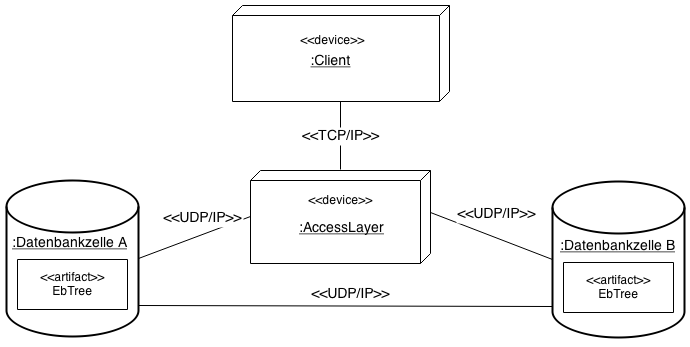
\includegraphics[width=0.8\textwidth]{bilder/uml_deployment_dia.png}
    \caption{Synchronisationsprozess}
\end{figure}
Eine weitere essentielle Komponente ist der \enquote{Accesslayer}. In diesem werden für neue Daten oder Veränderungen eindeutige \ac{ID}s erzeugt. Jedem neuen Datensatz wird eine eindeutige Nummer zugewiesen, die ihn adressiert, sowie eine (weitere?)Nummer, die seinen Stand wieder gibt. Neue \ac{ID}s steigen mit jeder weiteren Generierung. Wird ein neuer Datensatz eingefügt, oder verändert, sorgt der \enquote{Accesslayer} dafür, dass dieser adressiert, sowie an alle Datenbankzellen gesandt wird. Um auch hier eine möglichst hohe Ausfallsicherheit und eine Balancierung von Last zu gewährleisten, ist es möglich, dass mehrere \enquote{Accesslayer} parallel arbeiten. Die Koordination der unterschiedlichen \enquote{Accesslayers} ist eine weitere, umfangreiche Aufgabe, die im Rahmen dieser Arbeit nicht weiter erörtert wird.\\\\
\todo[inline]{Hinleitung zu Synchrobedarf da udp übertragung wegen performance} 
 Datenbanken -> in memory
Datenbanken system transparent
uml: Komponenten diagramm
Wo beschreibung der gundlegenden funktionen
grundlegende konzept mehrer Datenbanken mit gleichen Daten -> bedarf von synchronisation damit Daten konsistent bleiben

\section{Konzept der Datenbank}
\label{sec:DBConcept} 
%TODO in mermory!
Die grundlegende Idee der oben beschriebenen Datenbank ist, nicht wie in relationalen Datenbanken, Daten durch Tabellen zu gruppieren, sondern die Daten durch viele unterschiedliche Indexe zugänglich zu machen, je nachdem welche Kriterien für eine Gruppierung erforderlich sind. So kann jederzeit durch das Bilden von neuen Indexen auf neue Anforderungen an die Datenbank reagiert werden.\\\\
Neue Datensätze erhalten bei ihrer zentralen Erzeugung im \enquote{Access Layer} eine eindeutige, aufsteigende \ac{ID}. Die Nummer ist in allen Datenbanken gleich, verändert sich nie und adressiert den Datensatz, bis dieser gelöscht wird. Eine weitere Nummer, die \enquote{Change ID}, symbolisiert den Stand des Datums. Wenn das Datum angelegt wird, sind Identifikationsnummer und \enquote{Change ID} identisch. Wird der Datensatz verändert, wird diesem eine immer größer werdende \enquote{Change ID} zu gewiesen. Somit lässt sich leicht am Wert der \enquote{Change ID}  erkennen, ob Daten verändert wurden, oder sich noch ihrem Ursprungszustand befinden. Besonders vorteilhaft ist dies beim Vergleichen von Datensätzen in unterschiedlichen Datenbanken. Durch das Vergleichen der \enquote{Change ID} kann so sehr schnell ermittelt werden, welche von beiden aktueller ist, und somit der Unterschied ausgeglichen werden.\\\\
Für die \ac{ID}, als auch für die \enquote{Change ID}, wird eine eigener Index gepflegt. Hierfür wird der \ac{EB-Baum} verwendet (beschrieben in \autoref{sec:ebTreeGrundlagen}). Der \ac{EB-Baum} ist für diesen Zweck besonders gut geeignet, da dieser auf das Verwalten von nach Größe sortierten Ganzzahlschlüsseln optimiert ist. In die Datenbank eingefügte Datensätze werden in einem Container, dem \enquote{EbTreeDataObjekt}, gekapselt. Dieser enthält  die \ac{ID}, die aktuelle \enquote{Change ID}, sowie eine Referenz auf die Daten. Wird nun ein Datensatz in die Datenbank eingefügt, wird dieser mit der \ac{ID} in den dazugehörigen \enquote{ID-Baum} und mit der \enquote{Change ID} in den \enquote{Change ID-Baum} eingefügt. Das Blatt jedes Baumes hält somit die entsprechende Nummer und den Container. Es lässt sich somit leicht ermitteln, welche \enquote{Change ID} mit welcher \ac{ID} und umgekehrt verbunden ist. \\\\
Beim Verändern eines Datensatzes wird die alte \enquote{Change ID} aus dem \enquote{Change ID-Baum} gelöscht und die neue \enquote{Change ID} wieder eingefügt. Da der \ac{EB-Baum} seine Schlüssel der Größe nach von links nach rechts im Baum sortiert und neu erstellte Schlüssel immer größer werden, befinden sich neu eingefügte Elemente im \enquote{ID-Baum}, sowie kürzlich veränderte Elemente im \enquote{Change ID-Baum} ganz rechts in der Baumstruktur.\\\\
Soll ein Datum gelöscht werden, werden nicht einfach die damit verknüpften Nummern und der Datensatz gelöscht, da beim Löschen sichergestellt werden muss, dass das Datum aus allen Datenbanken entfernt wird. Das ist deshalb wichtig, da das jeweilige Datum sonst in dem nachfolgend beschriebenen Synchronisationsprozess einfach wieder hergestellt wird. Falls der Datensatz auf einer Seite der, an Synchronisation beteiligten Datenbanken, fehlt, er aber auf der anderen Seite vorhanden ist, lässt sich nicht mehr nachvollziehen, ob dieses Ungleichgewicht durch ein verlorenes Einfügen oder Löschen zu Stande gekommen ist. Außerdem lässt sich nicht mehr feststellen, ob das Element auf der einen Seite gelöscht, oder auf der anderen wieder hergestellt werden soll. Daher werden nur die Daten des \enquote{EbTreeDataObjekt} gelöscht und eine neue \enquote{Change ID} wird eingefügt. Das vollständige Löschen von \ac{ID} und \enquote{Change ID} aus beiden Bäumen, sowie das \enquote{EbTreeDataObjekt} erfolgt in einem gesonderten Löschprozess, der sicherstellt, dass diese Veränderung an jeder Datenbank vorgenommen wird.


\section{Synchronisation zwischen Datenbanken}
\label{sec:eBTreeSynchronisation}
\begin{figure}[h!]
        \centering
    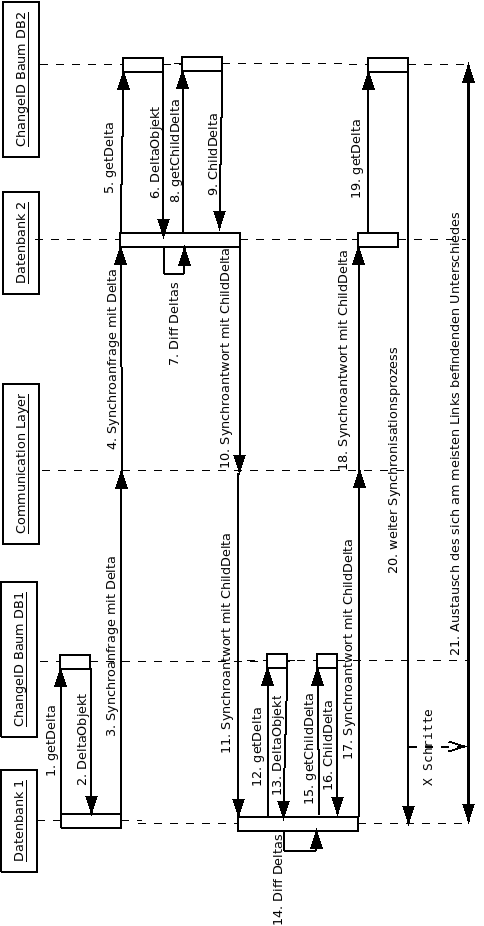
\includegraphics[width=1\textwidth]{bilder/SynchroProzess.png}
    \caption{Synchronisationsprozess}
\end{figure}
Durch ein Vergleichen der \ac{ID}s und \enquote{Change Ids} in den sich synchronisierenden Datenbanken kann einfach festgestellt werden, welche Daten fehlen und, falls ein Datensatz vorhanden, auf welcher Seite dieser aktueller ist. Ein Vergleichen der gesamten Datenbanken, gerade wenn diese unter hoher Last stehen und sehr viele Datensätze verwalten, beansprucht jedoch viele Ressourcen. Ab einem gewissen Grad von Last durch Operationen und Masse an Daten ist dies nur noch schwer umsetzbar. Ein komplettes Abgleichen nimmt in diesem Fall so viel Zeit in Anspruch, dass durch neue Operationen wieder ein Ungleichgewicht zwischen den Datenbanken entstehen würde.\\\\
Daher gilt es, eine Synchronisationsmethodik zu finden, die sowohl in der Lage ist, schnell kleine Unterschiede auszugleichen, als auch Datenbanken, die sich völlig verschiedenen Ständen befinden, über eine längere Zeitspanne zu synchronisieren.
Die \enquote{Change IDs}, die zum Vergleich während der Synchronisation gepflegt werden, werden in jeder Datenbank in einem \ac{EB-Baum} gehalten. Die Möglichkeit des Vergleichens von Zweigen unterhalb jedes Knotens ist daher von großem Vorteil. Um dies möglich zu machen, wird für jeden Knoten eine, den Zustand seiner beiden Kindobjekte repräsentierende Nummer, die \enquote{Knoten Change ID}, errechnet.
 Dazu werden die Nummern der Kindobjekte, \enquote{Change IDs} falls das Kind ein Blatt oder \enquote{Knoten Change ID} falls das Kind ein Knoten ist, durch eine \enquote{binäre XOR Operation} verbunden. Während des Synchronisationsprozesses senden sich beide Seiten sogenannte \enquote{Deltas}. Diese enthalten eine die Position des Deltaknoten beschreibenen Ganzzahl, die Bitebene des  Deltaknoten, der Bitebene des sich über dem Deltaknoten befindenden Elternknoten, sowie die deren Zustand wieder gebenden Nummern seiner Kinder.
Die übertragenen Werte beschreiben das logisch zusammenhängende Dreieck aus Knoten und zwei Kindern. Daher wird dieses als \enquote{Delta} bezeichnet.\\
\begin{wrapfigure}{r}{0.5\textwidth}
  \begin{center}
    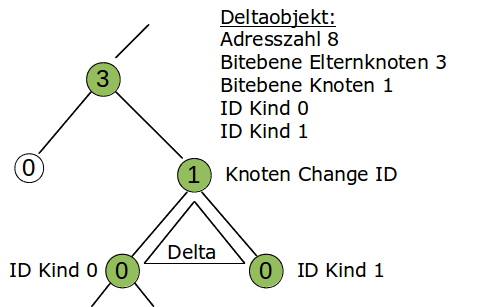
\includegraphics[width=.8\linewidth]{bilder/SynchroDelta.png}
  \end{center}
 \caption{Deltaobjekt}
\end{wrapfigure}
Durch die Ganzzahl, welche die Position des Deltas beschreibt, kann der Knoten, mit dem das Delta verglichen werden soll, in der anderen Datenbank gefunden werden. Bei der Lokalisierung des zu vergleichenden Knotens wird am obersten Knoten des Baumes begonnen und der Baum rekursiv durchlaufen. Je nachdem, ob 0 oder 1 in der Adresszahl an der binären Stelle der Bitposition des zu durchlaufenden Knoten gesetzt ist, wird das linke oder rechte Kindobjekt weiter behandelt. Dies wird solange wiederholt, bis die im Delta übergebene Bitebene des Deltaelternknoten unterschritten und der sich dort befindliche, zu vergleichende Knoten ermittelt ist.
Wird nach dem Vergleichen der Deltas festgestellt, dass die\enquote{Knoten Change IDs} der linken Knoten gleich und die der rechten Knoten ungleich sind, soll dieser Knoten ab jetzt nach rechts durchlaufen werden. Dazu wird in der binären Repräsentation des Adresswertes an der Bitstelle, die der Knoten darstellt, eine 1 gesetzt. Von nun an wird bei allen weiteren Durchläufen dieses Synchronisationsprozesses an diesem Knoten das rechte Kindobjekt behandelt.
Die Synchronisation kann von jeder Datenbank angestoßen werden. Eine Möglichkeit, dies zu koordinieren, ist, dass jede Datenbank zufällig in einem festgelegtem Zeitintervall zu synchronisieren beginnt. Es ist möglich, dass sich die Datenbank während des Synchronisationsprozess verändert. Die Synchronisation besteht aus zwei Phasen.  
\subsection{Synchronisation Phase 1} 
In der Ersten Phase gilt es, den Unterschied zu finden, der sich in beiden Bäumen am weitesten links befindet und somit den ältesten Unterschied zwischen den Datenbanken darstellt. Da im laufenden Betrieb auf der rechten Seite des Baumes viel Veränderung stattfindet, soll immer der Unterschied, der davon am weitesten Entfernt liegt, zu erst ausgeglichen werden. Daten, die sich oft verändern, sind sehr weit rechts im Baum zu finden. Somit besteht die Chance, dass sich möglicherweise verlorene Veränderungen bei einer erneuten Veränderung selbst ausgleichen.
Die Datenbank, die mit der Synchronisation beginnt, sendet ein Delta des höchsten Knotens, gekapselt in einer Synchronisationsanfrage, an die andere Datenbank. Diese lokalisiert den Knoten mit dem das Delta abgeglichen werden soll und vergleicht die Nummer des linken Kindobjektes des erhaltenen Deltas mit dem linken Kindobjekt des eigenen Knotens. Sind diese gleich, werden die rechten Kindobjekte verglichen. Wird dabei kein Unterschied erkannt, sind die Datenbanken synchron und der Synchronisationsvorgang ist abgeschlossen. Falls aber ein Unterschied lokalisiert wurde, wird darauf mit einem Delta, bestehend aus dem sich unterscheidenden Kindobjekt, geantwortet. Die Datenbanken spielen im Synchronisationsprozess mit dem Senden der Deltas eine Art \enquote{Ping-Pong}, bis der am weiten links liegende Unterschied gefunden wurde.\\\\
Beim Abgleichen der Deltas kommt es zu unterschiedlichen Vergleichsfällen, die vom Synchronisationsalgorithmus separat behandelt werden müssen.
\subsubsection{Unterschied Links/Rechts}
\label{sssec:SynchroDiffLeftOrRight}
Die Knotenstruktur in den \enquote{Change ID-Bäumen} beider Datenbanken ist bis zum ersten Unterschied identisch. Der Synchronisationsalgorithmus läuft Delta für Delta die Bäume entlang und navigiert dabei, nach links oder rechts abhängig davon Wo sich \enquote{Knoten Change Ids} unterscheiden, bis ein Blatt gefunden wird. Es besteht aber nun die Möglichkeit, dass sich an der Stelle, an der das Blatt gefunden wurde, im anderen Baum ein Zweig befindet, in dem das Blatt bereits vorhanden ist, \autoref{fig:Case1TreeB,B*}. Beim Vergleichen der \enquote{Change IDs} wird in diesem Fall ein Unterschied festgestellt, doch befindet sich dieser im Unterzweig der anderen Datenbank. Bevor dieser aber lokalisiert werden kann, wird in der Datenbank ohne den Unterzweig bereits dass Blatt gefunden. Daher wird sobald ein Blatt gefunden wird, dessen ID der anderen Seite mitgeteilt und dort geprüft ob diese bereits vorhanden ist. Falls das Blatt noch nicht vorhanden ist, werden nun die kompletten Daten des Blattes angefordert und eingefügt.\begin{wrapfigure}{r}{0.5\textwidth}
  \begin{center}
    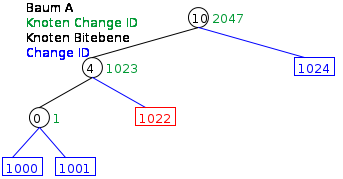
\includegraphics[width=0.9\linewidth]{bilder/Case1TreeA.png}
  \end{center}
 \caption{Baum A}
 \label{fig:Case1TreeA}
\end{wrapfigure} Ist das Blatt aber bereits im Baum, wird an die Position des Unterzweigs gelaufen und dort das Blatt betrachtet, welches sich am weitesten links befindet. Ist dieses nicht das gefundene Blatt, wurde der sich am weitesten links befindende Unterschied gefunden und der Datensatz zum Einfügen an die andere Datenbank gesandt. Ist das sich am weitesten links befindliche Blatt allerdings das Gefundene, ist der sich am weitesten links befindende Unterschied der nächste rechte Nachbar und kann ausgetauscht werden
\begin{figure}[h!]
  \begin{center}
    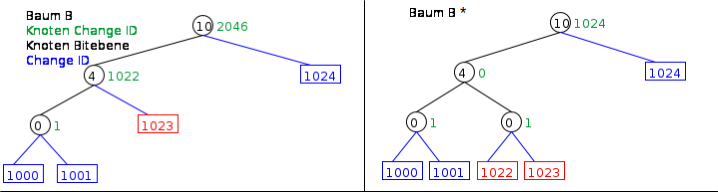
\includegraphics[width=0.9\linewidth]{bilder/Case B Baeume.png}
  \end{center}
 \caption{Baum B, B*}
  \label{fig:Case1TreeB,B*}
\end{figure}
\subsubsection{Behandeln von verschieden vielen Bitebenen} 
Abhängig davon, wie sehr sich die Bäume unterscheiden, so verschieden ist auch die Struktur an Knoten. Das führt zu folgender Problematik: Der älteste gesuchte Unterschied liegt links im Baum, doch fehlen ebenfalls andere, neuere Werte und somit auch die Knoten, die mit ihnen erzeugt werden. Ein einfaches \enquote{Delta Ping-Pong} Knoten für Knoten, und dabei Bitebene für Bitebene, ist daher nicht möglich. Auch ist von der Möglichkeit auszugehen, dass auf beiden Seiten Bitebenen fehlen. Dies führt zu einer Vielzahl an Möglichkeiten, in denen sich beiden Seiten unterscheiden können. Um die Lücken an Knoten zu erkennen und zu behandeln ist in den Deltaobjekten die Bitebene des Deltaknoten, sowie die Bitebene des oberhalb liegenden Elternknoten, enthalten.\\\\
Zu Beginn eines Synchronisationsschrittes wird im Baum der Knoten ermittelt, welcher sich unterhalb der Bitebene des Elternknotens des erhaltenen Deltas befindet. Dazu wird der Baum mit der Adresszahl solange durchlaufen, bis die Bitebene des betrachteten Knotens die Bitebene des Elternknotens des erhaltenen Deltas unterschreitet. Nun wird geprüft, ob die Bitebene des gefundenen Knotens gleich der Bitebene des erhaltenen Deltaknotens ist. Ist dies der Fall, wird mit der im oberen \autoref{sssec:SynchroDiffLeftOrRight}, Unterschied Links/Rechts, beschriebenen Prozedur verfahren. Unterscheiden sich die Bitebenen, führt dies zu zwei Möglichkeiten 
\begin{figure}[h!]
  \begin{center}
    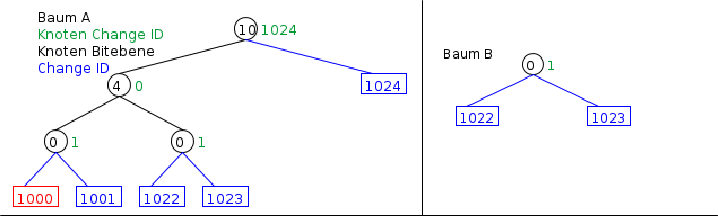
\includegraphics[width=0.9\linewidth]{bilder/case 2 a* B**.png}
  \end{center}
 \caption{Bäume mit verschieden vielen Bitebenen}
\end{figure}\\
Erste Möglichkeit: Die Bitebene des gefundenen Knotens ist kleiner als die des Deltaknotens. Zwischen den beiden Knoten befindet sich ein Loch, in dem sich noch nicht synchronisierte Blätter, sowie dazugehörige Knoten befinden. Diese sollen jedoch erst später vom Algorithmus repariert werden, da diese neuer sind und zuerst der älteste Unterschied behoben werden soll. Daher gilt es, das Loch zu überspringen. Dazu sendet die Seite mit dem tieferen Knoten ein spezielles Delta zurück, welches das nächst linke Delta unterhalb des erhaltenen Deltas anfordert. Dies wird solange wiederholt, bis auf beiden Seiten die selbe Bitebene erreicht ist, bzw. falls die kleine Bitebene im anderen Baum nicht vorhanden ist, ein Blatt gefunden wird. Ist auf beiden Seiten die gleiche Bitebene erreicht, können die Kinderobjekte, wie im obigen \autoref{sec:SynchroDiffLeftOrRight} beschrieben, verglichen werden.
Zweite Möglichkeit: Falls aber die Bitebene des gefundenen Knotens größer ist, als die des Deltaknotens, wird ein Delta aus dem gefundenen Knoten gebildet und zurück gesandt. Damit werden einfach die Seiten getauscht und der gerade beschriebene Fall tritt ein. Diese Methodik wird ebenfalls genutzt, um mit Synchronisation zu beginnen. Einer der Datenbanken wird ein manipuliertes Deltaobjekt gesandt. Dieses trägt als Absender die andere Datenbank. Die Werte der Bitebenen von Deltaknoten und Elternknoten sind negativ. Somit wird zuerst der oberste Knoten lokalisiert. Da dessen Ebenenbit positiv und somit größer ist, als der erhaltene negative Deltawert, wird der oberste Knoten als Delta an die andere Datenbank gesandt und ein Synchronisationsschritt beginnt. \\\\
\begin{figure}[h!]
  \begin{center}
    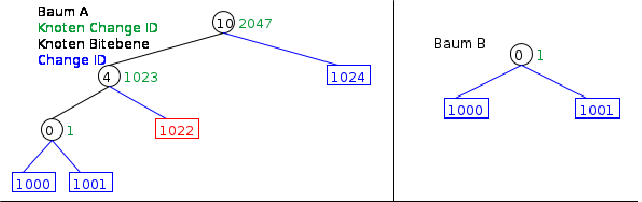
\includegraphics[width=0.9\linewidth]{bilder/case 2 A B1.png}
  \end{center}
 \caption{Bäume mit verschieden vielen Bitebenen}
\end{figure}
Ein weiterer Sonderfall tritt ein, wenn der Knoten und seine unter ihm liegenden Kinder des Baumes mit fehlenden Knoten im anderen Baum bereits vollständig enthalten ist und sich der gesuchte Unterschied oberhalb davon befindet. Während des Angleichens der Bitebenen werden keine \enquote{Change IDs} verglichen. Erst wenn auf beiden Seiten die selbe Bitebene erreicht ist, wird wieder nach Unterschieden geprüft. Wenn in diesem Fall links und rechts keine Unterschiede gefunden werden, erscheinen die Bäume synchron. Daher muss beim Überspringen des Bitebenenlochs überprüft werden, ob dieses bereits die selbe \enquote{Change ID}  hat wie der Knoten, bevor das nächst tiefere Delta angefordert wird . Ist dies der Fall, liegt der gesuchte Unterschied ganz links im rechten Kindobjektzweig, oder ist das Kindobjekt selbst.
\todo[inline]{Special case node nicht im anderen baum}

\subsection{Synchronisation Phase 2}
Nach Ablauf der ersten Synchronisationsphase ist die sich, in den \enquote{Change-ID Bäumen}, am weitesten Links befindende, unterscheidende \enquote{Change-ID} gefunden. Nun sendet die Datenbank in der sich diese befindet das gesamte \enquote{EbTreeDataObjekt} auf welches die \enquote{Change-ID} referenziert an die andere Datenbank in der die \enquote{Change-ID} nicht vorhanden ist. Durch die im \enquote{EbTreeDataObjekt} enthaltene \ac{ID} kann nun im  \enquote{ID-Baum} geprüft werden ob diese enthalten ist. Falls dies nicht der Fall ist die komplette Einfügeoperation des Datensatzes verloren gegangen und dieser muss nun nachträglich in beide Bäume eingefügt werden. Ist es Möglich die \ac{ID} zu lokalisieren ist dass \enquote{EbTreeDataObjekt} bereits in beiden Datenbanken vorhanden aber auf einem unterschiedlichem Stand. Nun gilt es durch einen Vergleich der beiden \enquote{Change-IDs} heraus zu finden auf welcher Seite der Datensatz aktueller ist und dies auszugleichen. Ist die erhaltene \enquote{Change-ID} größer als die Eigene wird der eigene Datensatz aktualisiert. Ist aber die erhaltene \enquote{Change-ID} kleiner kann der eigene Datensatz als Update an die andere Datenbank gesandt werden. Der Synchronisationsschritt ist abgeschlossen. Egal ob eine veraltete oder aktuelle  \enquote{Change-ID} gefunden wird jeder Synchronisationsschritt führt zum Ausgleich eines Unterschiedes.
	
\section{Architektur des Prototypen}
\begin{figure}[h!]
  \begin{center}
    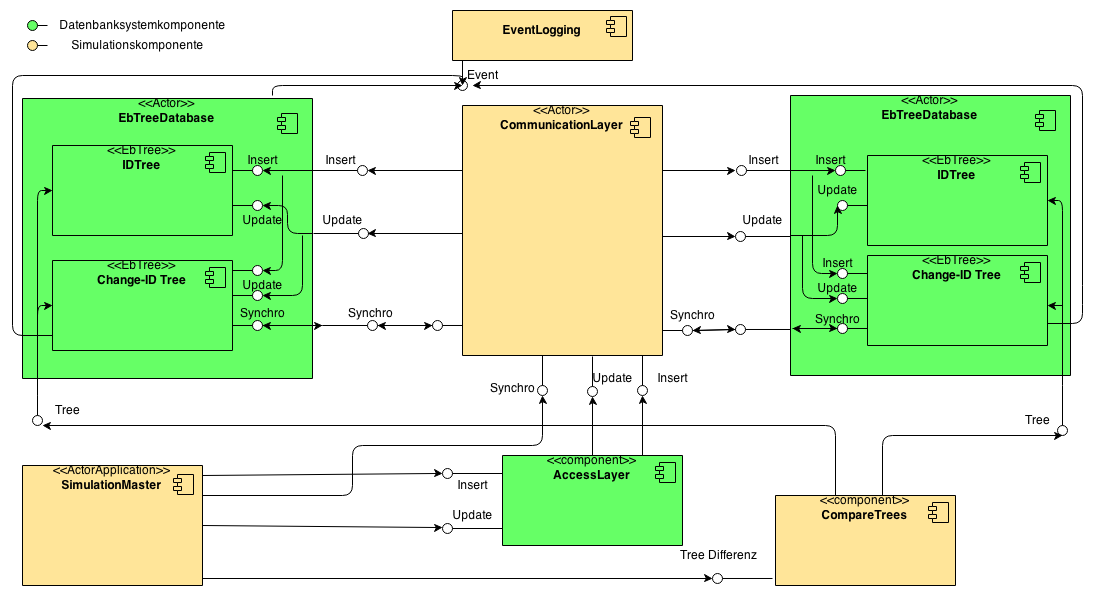
\includegraphics[width=1.0\linewidth]{bilder/prototyp_component_diagram.png}
  \end{center}
 \caption{UML Komponentendiagramm des Prototypen}
\end{figure}
\todo[inline]{ turn picture}
Der in dieser Arbeit erstellte Prototyp besteht grundlegend aus zwei Teilen. Zum einen besteht er aus den Komponenten des in \autoref{sec:DBConcept} beschriebenen Datenbankkonzeptes und der in \autoref{sec:eBTreeSynchronisation} erklärten Synchronisation zwischen zwei Instanzen der Datenbank. Zum anderen besteht er aus  einer Simulationsumgebung, mit welcher die Funktionalität des Datenbanksystems getestet werden kann. Die Synchronisation zwischen den einzelnen Datenbankinstanzen kann hier ebenfalls getestet und analysiert werden. Durch verschiedene Initialisierungen des Datenbanksystems, sowie dem Erzeugen von Last,  können verschiedene Szenarien erzeugt, und die Leistung des Systems bewertet werden. \\
Die Applikation ist zum Teil als Actorsystem umgesetzt. So wird jede Datenbank, sowie auch der \enquote{CommunicationLayer}, welcher als Bindeglied zwischen den Komponenten fungiert, durch einen Aktor repräsentiert.
Das Senden von Actornachrichten ähnelt dem Senden von IP-Paketen zwischen zwei Datenbanken an verschiedenen Standorten. Wann welche Nachricht in welcher Reihenfolge bei welcher Datenbank ankommt ist nicht vorhersehbar. Verlust, sowie Verspätung von Paketen und die daraus resultierende Asynchonität der Datenbanken, lassen sich so gut simulieren.
Zwischen den Datenbankaktoren befindet sich, als Teil der Simulationsumgebung, eine Kommunikationsebene. In dieser können Verlust und Verspätung von Paketen gesteuert werden.


\subsection{Datenbankkomponenten}
Der Prototyp setzt einen Teil der, in \autoref{sec:DBSystemConcept} beschriebenen, Komponenten um. Die Generierung von \ac{ID}s, welche neue Daten adressieren und den Stand von Aktualisierungen abbilden, werden in einer Basisimplementierung des \enquote{Accesslayer} generiert. Diese werden mit den Daten in einem \enquote{EbTreeDataObjekt} gekapselt und an alle Datenbankzellen gesandt. Jede Datenbankzelle wird durch einen Actor repräsentiert und kann Nachrichten mit neuen Daten, Änderungen oder Synchronisationsanfragen erhalten und senden. Im Rahmen dieser Arbeit werden zwei Datenbankzellen verwendet und Operationen wie Einfügen, Aktualisieren oder Löschen, sowie die Synchronisation zwischen beiden, getestet. Die Datensätze werden in einer Erweiterung des klassischen \ac{EB-Baum} gehalten.

\subsection{Simulationskomponenten}     
Die Komponenten der Simulationsumgebung setzen auf den Datenbankkomponenten auf. Zwischen den zwei Datenbankzellen und dem \enquote{Accesslayer} wird der \enquote{CommunicationLayer} zwischen geschoben. Der \enquote{CommunicationLayer} ist, wie die zwei Datenbankzellen, ein Actor. Werden neue Daten eingefügt oder aktualisiert, werden diese vom \enquote{Accesslayer} an den \enquote{CommunicationLayer} übergeben und an die zwei Datenbanken weiter verteilt. Auch die Synchronisation zwischen den beiden Zellen läuft durch den\enquote{CommunicationLayer}. Die Daten, die im Datenbankystem gekapselt in \enquote{EbTreeDataObjekten} oder \enquote{Deltaobjekten} versandt werden, werden als Nachrichten zwischen den Actoren versandt. Jede Nachricht passiert den \enquote{CommunicationLayer} und kann somit in diesem beeinflusst werden. So kann ein Prozentwert eingestellt werden, mit dem Pakete verloren gehen, um das Senden von UDP-Paketen zu simulieren. Auch die Verzögerung von Paketen kann hier simuliert werden. Neue Datensätze oder Aktualisierungen alter Daten werden in einer \enquote{Queue} abgelegt. Soll ein Paket verzögert werden, wird es lediglich, abhängig davon, wie stark die Verzögerung sein soll, weiter hinten eingereiht und somit später versandt. Durch Verlust und Verzögerung werden die Datenbestände in beiden Datenbanken verschieden. Je nachdem, wie hoch Verzögerung und Verlust im \enquote{CommunicationLayer} eingestellt sind, können in anderen Teilen der Simulationsumgebung die Auswirkungen auf das gesamte System und die Synchronisation ermittelt werden.\\\\
Startpunkt der Simulationsumgebung, als auch des gesamten Prototypen, ist der \enquote{SimulationMaster}. In dieser Komponente wird beim Start des Prototypen das Actorsystem initialisiert. Die beiden Datenbankzellen, \enquote{Accesslayer} und \enquote{CommunicationLayer}, werden instanziiert, deren Referenzen unter den Komponenten ausgetauscht und das gesamte Datenbanksystem, sowie die Simulationsumgebung selbst, initialisiert. Aufgabe des \enquote{SimulationMaster} ist es, zum einen das System zu initialisieren und zu starten, zum anderen darauffolgend eine Reihe verschiedener Simulationen zu ermöglichen. Während der Simulation werden Daten ausgewertet und diese in einem einer CSV-Datei gespeichert. Welche Simulation ausgeführt werden soll, kann von dem\_r Nutzer\_in  in einem einfachen \enquote{Kommandozeileninterface} ausgewählt werden. Je nach Simulation wird nun das Datenbanksystem mit Daten initialisiert und mit der Simulation begonnen. Während der Simulation kann der Inhalt der einzelnen Zellen verändert werden, um Last auf das Datenbanksystem zu simulieren. Der \enquote{SimulationMaster} generiert dazu neue Daten oder Änderungen und sendet diese, via des \enquote{AccessLayers}, an den \enquote{CommunicationLayer}. Dort wird nun entschieden, ob das Paket verloren geht oder verspätet wird. Anschließend wird dieses in der \enquote{Queue} abgelegt. Der \enquote{SimulationMaster} sendet in gewissen festgelegten Intervallen ein \enquote{Clocksignal}, welches dafür sorgt, dass die Pakete im ersten Feld der \enquote{Queue} versandt werden. Davon abhängig, wie hoch der Verlust oder die Verspätung von Paketen eingestellt ist, ergibt sich ein Unterschied zwischen den Zellen, der mit der Synchronisation ausgeglichen werden soll. Die Synchronisation der Datenbankzellen wird ebenfalls im \enquote{SimulationMaster} gestartet. Dazu wird an den \enquote{CommunicationLayer} die Nachricht gesandt, dass mit der Synchronisation eines Unterschiedes begonnen werden soll. In der Nachricht ist enthalten, welche Datenbank mit der Synchronisation beginnt. Der \enquote{SimulationMaster} wartet nun bis die Synchronisation eines Unterschiedes abgeschlossen ist und fährt dann mit der Simulation fort.\\\\

Um den Erfolg der Synchronisation und das Entstehen von Unterschieden bestimmen zu können, existiert die Komponente \enquote{TreeCompare}, mit welcher der Unterschied beider Datenbanken bestimmt werden kann. Um den Unterschied zu bestimmen, werden die \enquote{ID-Bäume} und \enquote{Change ID-Bäume} beider Datenbanken Blatt für Blatt verglichen und es wird gezählt, um wie viele Elemente sich wer unterscheiden. Beim Vergleichen der \enquote{ID-Bäume} kann festgestellt werden, um wie viele Einfügeoperationen und beim Vergleichen der \enquote{Change ID-Bäume} , um wie viele Aktualisiersoperationen sich beide Datenbanken unterscheiden.

%TODO eventlogging
%---------------------------------------------------------------------------------------------------------------------------------------------------
\chapter{Implementierung}
\todo[inline]{Realisierung/Umsetzung, Beschreibung der Implementierung, nicht des Programmcodes}
		\begin{enumerate}[1.]
			\item Umsetzung der Systemarchitektur
			\item Beschreibung und Besonderheiten der Implementierung
		\end{enumerate}

\section{EBTree} % teil gurndlage teil implementation
\label{sec:EbTreeImpl}
Die im Rahmen dieser Arbeit erstellte Scalaimplementierung des \enquote{Elastischen Binär Baums} orientiert sich zum einen an dem in Grundlagen~\ref{sec:ebTreeGrundlagen} beschriebenen Entwurf von Willy Tarreau\autocite{Tarreau}, als auch auf einer mehr spezifischen Basisumsetzung der Spinning Wheel GmbH.\\
In dieser wird bereits die enge Koppelung von Knoten und Blättern, der ursprünglichen C Implementation, aufgebrochen.\unsure{SPW c umsetzung mit blatt+node pointerns?}Die zuvor in \enquote{C structs} aufgebauten Knoten und Blätter wurden durch Java Klassen ersetzt und ihre gemeinsame Eigenschaften in einem Interface definiert. Basisfunktionen des Baumes wie einfügen, löschen und durchlaufen des Baumes waren hier ebenfalls vorhanden und wurden als Teil der Arbeit in Scala neu umgesetzt.\\\\
Eine besondere Anforderung an den Baum ist das die sortiert, verwalteten Schlüssel einzigartig sind und ein Einfügen von Duplikaten verhindert wird. Da das Verwalten von Duplikaten an sich möglich ist aber für das Funktionieren des Baumes nicht zwingend nötig wird ein einfügen Dieser, bei der folgend beschrieben Umsetzung, vermieden. \\
\subsection{Grundlegender Aufbau}
Der Baum selbst ist einer eigenen, generischen Klasse umgesetzt. Diese besteht aus den Funktionalitäten des Baumes, zwei \enquote{Case-Klassen}, repräsentativ für Knoten und Blätter, sowie einem \enquote{Trait} der deren gemeinsame Eigenschaften beschreibt. Der generische Typ der Klasse wird bei deren Instanziierung übergeben und legt den Datentyp der in den Blättern gespeicherten Daten fest. Somit kann der Baum jeder Art von Daten halten ohne verändert werden zu müssen.\\

Der \enquote{Trait} Child beschreibt was dass \enquote{Kind} eines Knoten können muss. Ganz gleich ob es sich hier um ein Blatt oder einen weiteren, einen neuen Zweig öffnenden, Knoten handelt. Festgelegt ist das ein jedes \enquote{Kindobjekt} eine Referenz auf ein \enquote{Elternobekt} haben muss und eine Methode die die eindeutig identifizierbare ID des Objektes zurück gibt. Die ID ist bei Blättern der Schlüssel mit dem das Blatt eingefügt wird und bei Knoten die \enquote{Node Change ID} welche zum vergleichen von Baumzweigen anderer Datenbanken bei der Synchronisation verwendet wird.\\

Durch den Einsatz von \enquote{Case-Klassen} kann durch \enquote{Pattern Matching} beim durchlaufen des Baumes sehr einfach geprüft werden welcher Klasse Kindelemente angehören und diese verarbeitet werden.\\

Die Aufgabe des Blatt \enquote{Case Klasse} ist sehr einfach. Sie hält die Referenz auf einen übergeben Datensatz und ist durch einen eindeutige Schlüssel identifizierbar. Knoten hingegen verfügen über mehr Logik. So kann dieser die in seiner Wurzel gespeicherten Kindobjekte, weitere Zweige oder Blätter, zurück geben oder neue anfügen. Durch sein Ebenenbit weiß ein Knoten auf welcher binären Ebene des Baumes er steht und kann in dem, bei einer Abfrage- oder Einfügeoperation, übergebenen Schlüssel an der entsprechenden Stelle nachschauen und seinen linkes oder rechtes Kindobjekt verarbeiten.

\begin{listing}[H]
	\begin{minted}[mathescape,
	               numbersep=5pt,
	               frame=lines,
	               framesep=1mm]{scala}
case class Node[T](myBit: Int) extends Child[T] {
    var myZero:				Child[T]  = _
    var myOne:				Child[T]  = _
    var nodeChangeID:	Long    	= _

    def bitOne(uid: Long): Boolean = ((uid & (1L << myBit)) != 0) && (myBit < 64)

    def getChild(uid: Long): Child[T] = bitOne(uid) match {
      case true => myOne;
      case false => myZero
    }
    def setChild(uid: Long, child: Child[T]) = {
      bitOne(uid) match {
        case true => myOne = child
        case false => myZero = child
      }
      child.myParent = this
    }
    override def getID(): Long = nodeStateID
  }	
	\end{minted}
	\caption{Umsetzung eines Knoten des \ac{EB-Baum}}
	\label{lst:Knoten EB-Baum}
\end{listing}

\subsection{Funktionalität des Baumes}
\subsubsection{Finden von Schlüsseln}
\label{sssec:FindKey}
Die Suche eines Schlüssel ist durch schlanke rekursive Funktion gelöst. Der zu suchende Schlüssel gibt einen Art binären Weg vor. So beginnt die Funktion am ersten Knoten des Baumes. Diesem wird der zu suchende Schlüssel übergeben. Der Knoten weiß durch sein Ebenenbit welche Stelle er in binären Repräsentation des Schlüssels ein nimmt. Je nach dem ob das Bit an dieser Stelle 0 oder 1 ist gibt er sein linkes oder rechtes Kindobjekt zurück. Nun kann via \enquote{Pattern Matching} unterschieden werden ob es sich bei diesem um einen weiteren Knoten handelt oder ein Blatt handelt. Ist das gefundene Objekt ein Blatt wird die Rekursion abgebrochen und das Blatt zurück gegeben. Falls ein Blatt mit dem gesuchten Schlüssel im Baum vorhanden ist wird dieses oder das Blatt mit am dem nächst kleinerem Schlüssel beim durch laufen des Rekursion gefunden. Falls das gefundene Objekt aber ein, einen weiterer einen neuen Zweig öffnenden, Knoten ist wird mit diesem die rekursive Funktion erneut aufgerufen bis ein Blatt gefunden wird.
\subsubsection{Einfügen eines neuen Blattes}
Beim einfügen eines neuen Blatt wird zunächst der Baum nach dem Schlüssel des neuen Blattes durchsucht. Falls der Schlüssel bereits vorhanden ist wird der neuen Datensatz im gefundenen Blatt eingefügt und der Alte zurück gegeben. So wird verhindert das Duplikate eingefügt werden können. Falls der Schlüssel nicht vorhanden ist und sich bereits Blätter im Baum befinden, liefert die für das Suchen von Blättern zuständige Methode dass Blatt dessen Schlüssel die ähnlichste binäre Repräsentation besitzt. Nun werden die Schlüssel des neuen und des gefundenem Blattes durch eine binäre Oder-Operation verknüpft und die Bitstelle des höchsten Bitunterschiedes ermittelt. Diese wird das neue Ebenenbit des Knoten der mit dem Blatt eingefügt wird. Nun muss die passende Ebene im bereits durch die Suche ermittelten Zweiges gefunden werden. Dazu wird das Ebenenbit des Elternknoten des gefundenen Blattes mit dem neue bestimmten Ebenenbit verglichen ist das Neue kleiner wurde die richtige Ebene gefunden andernfalls wird der Zweig Knoten für Knoten nach oben durchlaufen bis die passende Stelle gefunden ist. An dieser kann der neue Knoten samt Blatt eingehängt werden. Das Durchlaufen dieses Algorithmus stellt sicher das ein neuer Schlüssel stets an der richtigen Stelle eingefügt wird und der Baum aufsteigend von links nach rechts sortiert ist.
\subsubsection{Entfernen eines Blattes}
Soll ein Blatt aus dem Baum entfernt werden wird dieses zuallererst lokalisiert. Dazu wird der Baum nach dem Schlüssel des löschendem Blattes durchsucht. Nach dem Finden der Referenz des Blattes gilt es nun Blatt als auch den über dem sich befindenden Elternknoten zu entfernen. Dazu wird das andere Kindobjekt, ein Blatt oder ein weiterer Zweig, des Elternknoten an die Stelle des Elternknoten gehängt. Da nun keine Objekt mehr auf den Elternknoten referenziert wird dieser und das zu löschende Blatt durch den nächsten Durchlauf der \enquote{Garbage collection} gelöscht. Anschließend wird der Zähler der die Anzahl der Blätter im Baum hält dekrementiert und der Inhalt des gelöschten Blattes zurück gegeben.
\subsubsection{Erzeugen von Knoten Status IDs}
Das vergleichen von Blättern ist durch deren einzigartige, aufsteigenden Schlüssel einfach um zu setzen. Bei dem, in dieser Arbeit umgesetzten, Synchronisationansatz, ~\autoref{sec:eBTreeSynchronisation}, muss es aber möglich sein ganze Zweige unterhalb eines Knotens zu vergleichen. Daher besitzt der Baum eine Funktion die es ermöglicht für jeden Knoten eine Nummer, die \enquote{Knoten Status ID}, zu erzeugen die den Zustand seiner beiden Kinder repräsentiert.\\

Wird ein Blatt angefügt oder gelöscht werden die \enquote{Knoten Change ID} rekursiv nach oben bis zur Wurzel generiert.  Die Rekursion beginnt falls das Blatt neu eingefügt wurde am neu eingefügtem Knoten. Falls das Blatt gelöscht wurde am Knoten oberhalb des mit dem Blatt gelöschtem Knoten. Nun wandert die Rekursion Elternknoten für Elternknoten bis zur Wurzel des Baumes. Auf dem Weg wird für jeden Knoten eine neue \enquote{Knoten Change ID} generiert. Dabei werden die IDs seiner Kindobjekte einfach durch eine binäre XOR-Operation verknüpft und der Wert im Knoten gespeichert. Ist das Kindobjekt ein Blatt wird als ID der Schlüssel verwendet. Ist das Objekt ein Knoten seine bereits berechnete \enquote{Knoten Status ID}.

\subsubsection{Methoden zur Synchronisation und das Deltaobjekt}
Um die in \autoref{sec:eBTreeSynchronisation} beschriebene Synchronisation zu realisieren wird die nach Scala portierte Version des \ac{EB-Baum}es um zwei Methoden erweitert. Um den \enquote{Ping-Pong} artigen Austausch von Deltaobjekten zwischen den Datenbanken zu ermöglichen muss der Baum eine Methode besitzen die zu einem gegeben Deltaobjekt das nächste passende Objekt ermittelt. Zu Beginn wird in der Methode \enquote{nextDelta} der Knoten gesucht mit dem das erhaltene Delta verglichen werden soll. Dazu wird mit einer Rekursion der Baum von oben Knoten für Knoten durchlaufen bis entweder ein Blatt gefunden oder der Knoten ermittelt wurde dessen Bitebene unterhalb der Bitebene des erhaltenen Deltaelternknoten liegt. Die Navigation ob nach links oder rechts am Knoten abgebogen werden soll funktioniert gleich wie beim Suchen eines Blattes. Der Knoten hält dafür eine Methode bereit die zu einem gegebenen Schlüssel, hier die Adresszahl des erhaltenen Deltas, das entsprechende Kind zurück gibt. Dazu betrachtet der Knoten an der Stelle seines Ebenenbits in der binären Repräsentation des Schlüssels und entscheidet welches Kindobjekt zurück gegeben wird. Es wird solange ein nächstes Delta angefordert bis eine Seite ein Blatt entdeckt. Die nachfolgend beschrieben Vergleichslogik der Knoten entscheidet nur wie im Baum navigiert wird um am Ende ein Blatt zu lokalisieren.\\\\Wird nun ein Blatt gefunden wird dies der anderen Seite mitgeteilt. Dazu wird ein anderes speziell initialisiertes Deltaobjekt übertragen welches dieses als Blatt identifizierbar macht. Um die verschiedenen Zustände der Klasse Delta erstellen zu können besitzt diese ein \enquote{Companien Object} welches als \enquote{Factory} fungiert und je nach dem ob ein Blatt oder Knoten übergeben wird ein verschieden initialisiertes Delta zurück gibt. Bildet ein Delta ein Blatt ab sind die Werte für das rechte und linke Kindobjekt die \ac{ID} des Blattes, sowie als Knoten Bitebene -1. Die Adresszahl und die Bitebene des Elternknoten bleiben erhalten und ermöglichen es immer noch die Position des Blattes nachzuvollziehen. Die Klasse Delta besitzt eine Methode mit der abgefragt werden kann ob das Delta ein Blatt abbildet oder nicht.\\\\
\begin{listing}[H]
	\begin{minted}[mathescape,
	               numbersep=5pt,
	               frame=lines,
	               framesep=1mm]{scala}
def nextDelta(t:Delta):Delta = {
var node:Node[T] = rekFuncFindNode(myRoot.get.myZero) // Rekursion finden des Knotens
  if (node.myBit == t.to) { // Bitebene identisch vergleiche Kindobjekte
      if (node.myZero.getID() != t.l) {
        return Delta(t.id, t.to, node.myZero)
      }else if(node.myOne.getID() != t.r) {
        return Delta(t.id+(1L<<node.myBit), t.to, node.myOne); /
      }else{ return null } // trees synchronized
  }else if (node.myBit > t.to) {        // flip sides
      return  Delta(t.id, t.from, node); 
  }else { // node.myBit < t.to
      if (t.l == node.getID()) return new Delta(t.id+(1L<<t.to), 0 , 0, -1, -1)
      return  Delta(t.id, t.from, node.myBit, -1, -1) // request next left Delta
  }
}
	\end{minted}
	\caption{Vergleichslogik von erhaltenen Delta mit entsprechenden Knoten}
	\label{lst:DeltaComp}
\end{listing}
Wird aber in der beschriebenen Rekursion statt einem Blatt der erste Knoten unterhalb der Bitebene des Elternknoten des Deltas gefunden kann dieser mit dem erhaltenem Deltaknoten verglichen werden. Falls die Bitbene des Delta und Knoten identisch ist können die \ac{ID}s der Kindobjekte verglichen werden. Falls sich die linken \ac{ID}s unterscheidet wird aus dem linken Kindobjekt des Knotens ein Delta gebildet. Falls diese aber gleich sind werden die \ac{ID}s rechten Kindobjekte verglichen. Sind auch diese gleich ist der Baum synchron. Die Methodik des Synchronisationsalgorithmus stellt hierbei sicher dass dieser Fall nur im obersten Knoten eintreten kann. Sind die rechten Kindobjekte unterschiedlich wird in der Adresszahl in binären Stelle der Bitebene des Knotens das Bit gesetzt. Dazu wird zur Adresszahl der Wert addiert der das entsprechende Bit setzt. Wurde links oder rechts eine Differenz erkannt wird aus dem entsprechendem Kindobjekt ein Delta erstellt und zurück gegeben. Das Kindobjekt wird durch das Interface Child abgebildet und kann Knoten oder Blatt sein. Die \enquote{Factory Methodik} der Deltaklasse bildet daher automatisch das passende Delta egal ob das Kindobjekt ein Blatt oder Knoten ist und liefert dieses zurück.\\\\
Das in \autoref{sec:eBTreeSynchronisation} \enquote{Behandeln von verschieden vielen Bitebenen} beschrieben Problem wenn sich die Bitebene des Deltaknoten und gefundene Knoten unterscheiden wird in der Implementation wie folgt umgesetzt: Ist die Bitebene des Knoten größer wird der gefundene Knoten wird aus diesem ein Delta gebildet und zurück gegeben. Wird dieses Delta dann im anderen Baum verarbeitet ist es kleiner als der Knoten. Wenn die Bitebene des Knoten kleiner ist als die des Deltas wird vom anderen Baum das nächste vom erhaltenen Delta gesehene tiefere linke Delta angefordert. Dazu werden die Felder für die \ac{ID}s der Kinder auf minus Eins gesetzt. Die Adresszahl und die Ebene des Deltaelternknoten bleiben gleich. Somit wird beim Rekursiven suchen des Knotens im anderen Baum dort wieder der Deltaausgangsknoten gefunden. Durch eine Abfrage vor dem Vergleich der Bitbenen wird erkannt das die Felder der Kinder mit minus Eins belegt sind und somit erkannt das dass nächste linke Delta unterhalb des Knotens angefordert wurde. Dies wiederholt sich bis die Bitbenen identisch und ein Vergleich der Kinder möglich ist, die Bitebene des angeforderten Deltaknotens kleiner als die eigene Bitebene des Knotens ist und wieder Seiten getauscht werden oder ein Blatt gefunden wird.\\\\
Am Ende der in \autoref{sec:eBTreeSynchronisation} beschrieben Logik wird entweder ein Blatt gefunden dass nicht in beiden Bäumen vorhanden ist oder die Synchronisation beendet da die Bäume gleich sind. Wird ein sich unterscheidendes Blatt gefunden und an die andere Datenbank gesendet muss geprüft werden ob sich dieses wirklich nicht bereits vorhanden ist. Dies ist notwendig auf Grund des in \autoref{sec:eBTreeSynchronisation} \enquote{Unterschied Links/Rechts} bereits beschriebenen Sonderfalls, siehe \autoref{fig:Case1TreeB,B*}. Bei diesem befindet sich das vermeintlich unterscheidende Blatt im anderen Baum nur in einem tiefer liegendem Zweig. Daher wird eine weitere Methode, \enquote{checkIfLostLeafIsFound}, bereit gestellt die prüfen kann ob das Blatt im Baum vorhanden ist oder nicht. Wenn dies der Fall ist kann die Methode das sich am weitesten links im Zweig befindende Blatt lokalisiert. Dies ist mit Sicherheit nur auf einer Seite vorhanden ist da auf der anderen an der Stelle des Zweiges nur ein Blatt ist und somit alle Blätter außer diesem einen fehlen. Die Methode bedient sich zu beginnt der in \autoref{sssec:FindKey} \enquote{Finden von Schlüsseln} beschrieben Logik. Kann zu dem gegebenen Schlüssel kein Blatt gefunden werden ist dieser der gesuchte sich der am weitest Links befindende Unterschied und der erhaltene Schlüssel wird zurück gegeben. Ist der Schlüssel aber im Baum enthalten wird zuerst der Knoten gesucht der sich im Baum an der Stelle des Blattes befindet. Da im erhaltenen Deltaobjekt noch die Adresszahl und die Bitebene des Elternknoten des erhaltenen Blattes enthalten ist kann der Baum wieder rekursiv von oben durchlaufen bis der Zweig lokalisiert ist. Der Zweig wird nun bis zum sich am weitesten links befindenden Blattes durchlaufen. Nun muss nur geprüft werden ob dieses Blatt dass bereits als Deltaobjekt erhaltene Blatt ist. Ist dies der Fall wird das nächste rechte Blatt zurück gegeben. Falls nicht das gefundene sich ganz links im Zweig befindliche Blatt. 
\subsubsection{Durchlaufen des Baumes}

%TODO durachlaufen des Baumes



\section{EbTreeDatabase}
\subsection{Grundlegender Aufbau}
Die Klasse \enquote{EbTreeDatabase} implementiert den in \autoref{sec:DBConcept} beschriebenen Aufbei einer Datenbankzelle. Sie erweitert die die Klasse Actor des \enquote{Akka Actor toolkit} \autocite{Akka}. Die Kommunikation mit der Datenbankzelle erfolgt somit ausschließlich durch das Senden von Nachrichten die Klasse verfügt über keine öffentlich erreichbaren Methoden. Die Datenbank besitzt eine \enquote{Mailbox} in der erhaltene Nachrichten abgelegt werden. In der zu überschreibende Methode \enquote{receive} werden die Nachrichten definiert die von der Datenbank verarbeitet werden sollen. Dies ist über die in Scala Logik des \enquote{Pattern Matching} realisiert. Erhaltene Daten werden in diesem Datenbankprototyp in zwei Indexen gehalten. Dazu werden die Daten in der Klasse \enquote{EbTreeDataObject} gehalten. Diese verfügt über ein Feld für die \ac{ID}, ein Feld für die \enquote{Change-ID} sowie einer Referenz auf die eigentlichen Daten. Der Datenbankklasse wir bei ihrer Instanziierung ein Typ übergeben welcher den Typ der eigentlichen im  \enquote{EbTreeDataObject} gekapselten Daten festlegt. Durch diese Logik eines generischen Types kann jede Art von Daten in der Datenbank abgelegt werden. Die beiden Indexe in dieser Basisumsetzung der Datenbank werden durch den in \autoref{sec:EbTreeImpl}
\ac{EB-Baum} realisiert. Die Datenbank hält zudem Referenzen zu den anderen im System existierenden Datenbankzellen,welche in einer Liste aus Actorreferenzen gehalten werden, sowie einer Referenz auf den für die Simulation im Prototypen essentiellen \enquote{CommunicationLayer}.\\

\subsection{Verarbeitung von Nachrichten}
Bei den in der Datenbank verarbeiten Nachrichten handelt es sich nicht wie der Name Nachricht erst vermuten lässt um Text sondern jede Nachricht wird durch eine eigene \enquote{Case Klasse} oder ein \enquote{Case Objekt} abgebildet. Somit können Nachrichten einen Zustand besitzen und kapseln im Actorsystem versandte Daten. Die versandten Nachrichten in diesem Prototyp sollen das senden von UDP-Pakten nachbilden. Daher soll jede Nachricht ein Ziel als Absender besitzen. Der Trait \enquote{EBTreeMessage} soll dies realisieren. Er definiert hierfür zwei Felder des Typs \enquote{ActorRef}. Nachrichten die innerhalb des Datenbanksystems augetauscht werden erweitern diesen Trait und sind daher adressierbar.

\subsubsection{Nachricht: Einfügen}
Die \enquote{Case Klasse} \enquote{InsertNewObject} wird genutzt um neue Datensätze in die Datenbank einzufügen. Diese beinhaltet ein im \enquote{AccesLayer} erzeugtes \enquote{EbTreeDataObject}. Dieses wird zuerst mit seinem Attribut \enquote{uID} in den als Index für die \ac{ID}s verwendeten \ac{EB-Baum} eingefügt und anschließend mit dem Attribut \enquote{changeId} in den \enquote{Change-ID Baum}.
\subsubsection{Nachricht: Aktualisieren}
Das Aktualisieren eines bereits enthalten Datensatzes wird durch eine Nachricht der \enquote{Case Klasse} \enquote{UpdateObject} aufgerufen. Zu erst wird mit dem Attribut \enquote{uID} geprüft ob das \enquote{EbTreeDataObject} bereits in der Datenbank vorhanden ist. Ist dies der Fall wird dem gefundenen \enquote{EbTreeDataObject} die alte \enquote{Change-ID} abgefragt und mit dieser das entsprechende Blatt aus dem \enquote{Change-ID Baum} und das Blatt aus dem \enquote{ID-Baum} entfernt. Das neue \enquote{EbTreeDataObject} kann nun in beide Indexe eingefügt werden.
\subsubsection{Nachricht: Löschen}
Soll ein Datum aus der Datenbank gelöscht werden wird dieses wie in \enquote{Nachricht: Aktualisieren} durch ein neues \enquote{EbTreeDataObject} ausgetauscht bei dem die Payload keine Daten enthält. Gelöschte Datensätze werden in den beiden Indexen weiter gepflegt um ein Wiederherstellen durch die Synchronisation zu verhindern, siehe \autoref{sec:DBConcept}. Das Löschen wird durch den Erhalt der \enquote{Case Klasse} \enquote{RemoveObject} aufgerufen.
\subsubsection{Nachricht: Synchronisation}
Der Synchronisationsdialog zwischen den sich synchronisierenden Datenbankzellen erfolgt durch das Senden der \enquote{Case Klasse} \enquote{Synchronize}. Diese enthält das zum Verarbeiten in den eigenen Indexen benötigte \enquote{Deltaobjekt} der anderen Datenbank. Zu erst wird geprüft wie viele Elemente in der eigenen Datenbank vorhanden sind, da für die Funktionaltät Synchronisationsmethodik mehr als ein Datensatz vorhanden seien muss. Ist dies der Fall wird die Synchronisationsnachricht weiter verarbeitet, ansonsten diese verworfen. Anschließend wird geprüft ob das erhaltene Deltaobjekt ein bereits gefundenes sich unterscheidendes Blatt oder einen zu vergleichenden Knoten repräsentiert. Wird festgestellt dass das dieses einen Knoten darstellt kann dieser der vergleichenden Synchronisationsmethodik des \enquote{Change-ID Baumes} übergeben und  von dieser zurück gegebene Deltaantwort zurück gesandt werden. Versandte Synchronisationsnachrichten werden zuerst adressiert und dann an den \enquote{CommunicationLayer} gesandt der diese dann anhand der Adressierung weiter \enquote{routed}. \\\\
Stellt sich heraus dass das erhaltene Delta aber ein sich möglicherweise unterscheidendes Blatt repräsentiert, kann nun, mit der in \autoref{sec:EbTreeImpl} \enquote{Methoden zur Synchronisation und das Deltaobjekt} beschrieben Methode \enquote{checkIfLostLeafIsFound} des \enquote{Change-ID Baumes}, geprüft werden ob dieses in in der eigenen Datenbank bereits vorhanden ist oder eingefügt werden soll. Falls das Blatt vorhanden ist wird vom Baum eine \enquote{ChangeID} zurück gegeben die auf einen Datensatz repräsentiert der sich nicht in der anderen Datenbank befindet. Daher kann nun der komplette Datensatz an die andere Datenbank gesendet werden. Dieser wird in der eignen Datenbank lokalisiert, in der \enquote{Case Klasse} \enquote{CheckLeaf} gekapselt und über den \enquote{CommunicationLayer} an die andere Datenbankzelle geschickt.
Ist die im Deltaobjekt enthaltene \enquote{Change-ID} nicht vorhanden wird der gesamte Datensatz angefordert. Dazu wird die \enquote{Case Klasse} \enquote{RequestEbTreeDataObject} verwendet. Ihr ist das Delta angehängt mit dem in der anderen Datenbank das Datum lokalisiert und in \enquote{CheckLeaf} eingepackt zurück gesandt wird.\\\\
Wird eine Nachricht des Types \enquote{CheckLeaf} erhalten gilt es nun das in ihr enthaltene \enquote{EbTreeDataObject} in beide Indexe einzufügen. Als erstes wird geprüft ob sich dieses bereits in der Datenbank befindet. Ist das Datum nicht im \enquote{ID-Baum} vorhanden ist der gefundene Unterschied durch eine verloren gegangene \enquote{InsertNewObject} Nachricht zustande gekommen und das \enquote{EbTreeDataObject} kann wie in vorherigen Absatz \enquote{Nachricht: Einfügen} in beide Indexe eingefügt werden.
Ist aber ein Blatt mit Referenz auf den Datensatz im \enquote{ID-Baum} vorhanden wurde der Unterschied zwischen beiden Datenbanken durch ein verloren gegangenes \enquote{UpdateObject} oder \enquote{RemoveObject} verursacht. Ein Vergleich der \enquote{Change-IDs} des als Nachricht enthaltenem, mit sich in der eigenem Datenbank befindlichem \enquote{EbTreeDataObject} ist daher nötig um festzustellen welcher von beiden Datensätzen veraltet ist. Ist die eigene \enquote{Change-ID} kleiner wird der Datensatz eingefügt. Dazu wird sich der im Absatz \enquote{Nachricht: Aktualisieren} bereits implementierten Funktionalität bedient und der Datensatz gekapselt in einer \enquote{UpdateObject} Nachricht den den Datenbankaktor selbst gesandt. Falls aber die eigene \enquote{Change-ID} größer ist wird der Datensatz in einer \enquote{CheckLeaf} Nachricht der anderen Datenbankzelle geschickt. Um mögliche Fehler lokalisieren zu können wird auch auf Gleichheit der \enquote{Change-IDs} geprüft. Dieser Fall darf im Synchronisationsalgorithmus nicht auftreten und wird an dieser Stelle mit einem Eintrag im später beschriebenen \enquote{EventLogging Obejkt} erfasst.

\section{Accesslayer}
Aufgabe des \enquote{AccessLayers} ist das Erzeugen von einzigartigen Identifikationsnummer zur addresierung von Datensätzen. Wird ein Datum in das Datenbanksystem eingefügt so wird es zu erst einem \enquote{AccesLayer} übergeben. Dieser erzeugt nun die, bis die Daten gelöscht werden, sich nicht verändernde Identifikationsnummer und sendet beide gekapselt in einem \enquote{EbTreeDataObject} an alle Datenbankzellen. Zu diesem Zeitpunkt ist die \enquote{Change-ID} identisch mit der generierten \ac{ID} was zu erkennen gibt dass der Datensatz sich in seinem Ursprungszustand befindet. Verändert sich ein Datensatz wird dieser wieder an den \enquote{AccessLayer} übergeben und eine neue \enquote{ChangeID} generiert und das veränderte Objekt abermals an alle Zellen gesandt.\\\\
Um sicher zustellen das eine sehr große Menge an Datensätzen eindeutig adressiert werden können wird für die Schlüssel der Datentyp \enquote{Long} verwendet. Die Notwendigkeit eines großen Schlüssels entsteht auch durch den Prozess des Bildens der \enquote{Knoten Change-IDs} in den Bäumen. Diese werden durch eine binäre XOR-Operation verbunden und bei zu kleinen Schlüsseln steigt die Wahrscheinlichkeit dass sich beim Verrechnen unterschiedlichen Zahlen die selben \enquote{Knoten Change-IDs} ergeben. Daher sinkt mit der Größe des Schlüssels die Warscheinlichkeit dieses Problems, siehe \autoref{sec:XorError}.\\\\
Der Schlüssel wird aus mehreren verschieden langen Teilen zusammen gesetzt, die am Ende einen 64 Bit langen Longwert ergeben. Da jeder neu erzeugte Schlüssel einen größeren Wert als alle vor ihm generierten besitzen muss ist das erste Teil des Schlüssel ein Zeitwert. Dazu werden 40 der 64 Bit verwendet. Da es aber möglich ist, gerade wenn mehrere \enquote{AccessLayers} parallel arbeiten, das zwei Datensätze im selben Zeitfenster adressiert werden erhält der Schlüssel noch eine acht Bit lange Sequenznummer und sowie einen sechzehn Bit lange Zufallszahl. Beim Bilden der ID werden die Binärwerte der Zahlen aneinandergereiht und der sich daraus ergebene Binärwert wieder in einen 64 Bit Longwert umgewandelt.

\section{CommunicationLayer}
Der \enquote{CommunicationLayer} wird als Teil der Simulationsumgebung zwischen die Komponenten des Datenbanksystems geschoben. Die gesamte Kommunikation des Datenbanksystems durchläuft diese Komponente und wird von ihr an die entsprechenden Ziele geroutet. Da jede Nachricht die zwischen den Datenbankzellen verschickt wird, durch die Erweiterung des Traits \enquote{EBTreeMessage}, ein Ziel und Empfänger besitzt können alle Nachrichten an den \enquote{CommunicationLayer} gesandt  und von diesem weiter verteilt werden. Fehler wie Verlust und Verzögerung von Paketen wie sie in einem realen verteilten Datenbanksystem bei der Verwendung von UDP auftreten, können an dieser Stelle einfach simuliert werden. Der Klasse wird bei Ihrer instanziierung ein Prozentwert mit welcher Nachrichten verloren gehen, sowie ein Prozentwert wie wahrscheinlich eine Verzögerung ist mit übergeben. Wird nun ein Paket eingefügt prüfen zwei Methoden ob ein Fehlerfall eingetreten ist. Dazu wird in jeder Methode eine Zufallszahl zwischen Null und Einhundert erzeugt ist diese kleiner als der jeweilige gegeben Prozentfehlerwert geht die Nachricht verloren oder wird um einen Zyklus verzögert.\\\\
Um Verzögerung von Last zu simulieren werden Nachrichten die einen neuen Datensatz einfügen oder aktualisieren zuerst in einer Liste abgelegt. Erst wenn eine \enquote{Clock-Nachricht} vom \enquote{SimulationMaster} eintrifft werden alle Nachrichten die sich im Kopf der Liste befinden ausgeliefert. Tritt der Fall ein das eine Nachricht verzögert werden soll wird diese einfach an zweiter Stelle in die Liste gelegt und erst eine \enquote{Clockintervall} später ausgeliefert.\\\\
Die beider Synchronisation versandten Pakete passieren ebenfalls den \enquote{CommunicationLayer} werden aber nicht verzögert oder verworfen. Dies ist aber an dieser Stelle durch das Konzept der Klasse einfach umzusetzen. Soll die Synchronisation gestartet werden wird dem \enquote{CommunicationLayer} die \enquote{Case Klasse} \enquote{StartSynchro} geschickt und dieser sendet dann ein manipuliertes Deltaobjekt an eine der Datenbankzellen um die Synchronisation zu starten.

\section{SimulationMaster}
actorsystem
initiliserung der komponenten
user ui
initilisierung der datenbanken
testdurchlauf
csv der testdaten

\section{Vergleichen von Bäumen}
\label{sec:DiffTrees}
Um den Erfolg der Synchronisation überprüfen zu können, wird eine Klasse benötigt dies es ermöglicht zwei Datenbanken zu vergleichen. Die Klasse \enquote{TreeCompare} vergleicht dazu alle Elemente beider Bäume und ermittelt um wie viele Einfüge- und Aktualisierungsoperationen sich die Datenbanken unterscheiden. Dabei wird das umgesetzt, was der, in dieser Arbeit beschriebene, Synchronisationsalgorithmus zu vermeiden versucht: Das aufwendige Vergleichen aller Blätter. Bei ihrer Instanzierung werden die Referenzen beider Datenbankzellen übergeben. Durch das Senden der \enquote{Case-Klassen}: \enquote{GetChangeIdTreeRequest} und \enquote{GetuIdTreeRequest} werden den Datenbankzellen die Referenzen auf die Indexbäume entnommen. Anschließend werden die  \enquote{ID-Bäume} und \enquote{ChangeID-Bäume} beider Datenbanken verglichen. Dabei wird folgendermaßen vorgegangen: Es wird Blatt für Blatt durch die Bäume iteriert. Dabei werden die IDs der Blätter von Baum A mit denen von Baum B verglichen, wobei Differenzen gezählt werden. Dazu wird jeweils die Referenz der ersten Blätter der Bäume in einem Zeiger gespeichert und diese miteinander verglichen. Der Zeiger des kleineren Wertes springt dann solange zum nächsten Blatt bis der Wert entweder gleich oder größer als der Wert des anderen Blatt ist. Der andere Zeiger wartet bis die Werte entweder gleich oder sein Wert kleiner geworden ist. Sind die Werte gleich wechseln beide Zeiger zum nächsten Blatt. Wird der Wert des wartenden Zeiger überschritten iteriert nun dieser durch seine Blätter bis wieder größer oder gleich dem anderen Wert ist. So werden beide Bäume komplett durchlaufen und bei jedem Unterschied der Zähler \enquote{diff} inkrementiert. 

\section{Erfassen von Ereignissen}
Das Erfassen der Anzahl verschiedener Ereignisse ist ebenfalls eine Funktionalität die während der verschiedenen Simulationen möglich seien muss. Daher existiert das Objekt \enquote{EventLogging}. Da es sich um ein Scala Objekt handelt, ähnlich der statischen Klasse in Java, ist es nicht nötig ist, wie beim klassischem \enquote{Logging}, Instanzen zu erstellen oder bereits erstellte herum zu reichen. Das Objekt enthält eine \enquote{Map} als Attribut. Tritt nun ein zu erfassendes Ereignis ein wird einfach ein Key/Value Paar gespeichert. Der Key ist dabei ein bezeichnender String und das Value die Anzahl wie oft das Ereignis hinzugefügt wurde.

%---------------------------------------------------------------------------------------------------------------------------------------------------
\chapter{Test}
\todo[inline]{Testarten, Testkriterien, Testumgebung, Testergebnisse}

 Testkriterien und Szenarien
Demonstration der Funktionalität
Auswertung der Ergebnisse\\

Um die Funktionalitaet des, in \autoref{sec:eBTreeSynchronisation} beschriebenen, Synchronisationsalgorithmus, innerhalb des in \autoref{sec:DBSystemConcept}	beschriebenen verteilten Datenbanksystems, zu beweisen und zu testen werden hier folgend beschriebene Test durch geführt. Durch das Verwenden des Scala Testframeworks \enquote{Funsuite} wird die Funktionalität einzelner Programmkomponenten des Prototypen getestet. Die Funktionalität des Synchronisationsalgorithmus wird allerdings in der eigens erstellen Simulationsumgebung getestet und analysiert. Dabei wird in statische und dynamische Tests unterschieden. Bei den statischen Testfällen wird das System auf einen je nach Test verschiedenen Stand gebracht und anschließend durch die Synchronisation ausgeglichen. Bei den dynamischen Tests ist dies ebenso jedoch wird während des Synchronisationsprozesses das Datenbanksystem  weiter durch einfügen neuer und verändert alter Datensätze verändert. Ziel bei beiden ist es die zu messen wie sich die Performance des Algorithmus bei unterschiedlich Gegebenheiten verhält und zu ermitteln ob, sowie wie lang dieser erfolgreich Konsistenz im Datenbanksystem herstellen kann. was wird gemesen deltapks pro
Begriffserklärung:
\begin{description}
	\item[TPS Transaktionen pro Clock]
	\item[(delta+request)Synchropkt pro Clock	]
	\item[Synchronisationsnachrichten] Alle Nachrichten die bei der Synchronisation versandt werden wie Deltapakete, Anfragen nach Datensätzen, sowie der Datensatz der auf der anderen Seite fehlt.
	\item[Synchronisationszyklus] Vollständige Prozedur des Ausgleichen eines Unterschiedes zwischen den Datenbanken. Beginnt mit dem senden des obersten Deltapaketes einer Datenbankzelle und endet mit dem Austausch eines Datensatzes. Je nach dem wie sich die Struktur der zu vergleichen Baumstrukturen unterscheidet benötigt ein Zyklus mehr oder weniger Synchronisationsnachrichten.
\end{description}


\newpage
\section{Statische Tests}
\subsection{Knoten Change-IDs durch XOR}
\label{sec:XorError}
Das Erzeugen der \enquote{Knoten Change-IDs} erfolgt, wie in \autoref{sec:eBTreeSynchronisation} beschrieben, durch die Verknüpfung der IDs der Kinderobjekte des Knotens durch eine \enquote{binäre XOR Operation}. Jedoch kann der Fall eintreten dass mit dieser Operation aus verschiedenen Werten die selbe Zahl erzeugen erzeugt. Dies führt so folgender Problematik: Bei der Generierung der \enquote{Knoten Change-IDs} ist es möglich das in verschiedenen Datenbankzellen für Knoten die selbe \enquote{Knoten Change-ID}  errechnet wird aber ihre Kindobjekte sich unterscheiden. Befinden sich diese Knoten in den Bäumen an der selben Stelle stellt der Synchronisationsalgorithmus bei deren Vergleich fest dass die IDs identisch sind und überspringt somit die darunter liegenden Blätter und Zweige. Dies hat zur Folge das ganze Teile der Bäume nicht verglichen werden und dort liegende Unterschiede nie Erkannt werden. Je größer und je verschiedener die Schlüssel sind um so geringer ist die Wahrscheinlichkeit dass dies passiert. Aber mit der Anzahl der eingefügten Datensätze steigt auch wieder die Wahrscheinlichkeit dass es zu dieser blockierenden Fehlfunktion kommen kann. Dieser Test soll daher ermitteln wie weit, bei verschieden großen Schlüsseln, die Funktionalität, unter Verwendung der \enquote{binäre XOR Operation} zum generieren \enquote{Knoten Change-IDs}, der Synchronisation gewährleistet werden kann.\\\\
Das die beschriebene Blockade eingetreten ist lässt sich nur durch ein vollständiges Vergleichen der Bäume feststellen. Dazu wird der in \autoref{sec:DiffTrees} beschrieben Algorithmus verwendet. Nach jedem die gesamte Synchronisation abgeschlossen ist wird die Anzahl der Unterschiede zwischen den Datenbanken bestimmt. Wird nach Abschluss der gesamten Synchronisation ein Unterschied bestimmt ist der Fehlerfall eingetreten. Die Synchronisation stellt an diesem Punkt fest dass die IDs der Kindobjekte des obersten Knoten auf beiden Seiten identisch sind und somit die gesamte Synchronisation abgeschlossen ist. \\\\
In diesem Test werden folgende Schlüsselgrößen getestet:
\begin{description}
	\item[48 Bit] besteht aus 32 Bit Zeitstempel in Sekunden, sowie 16 Bit Zufallszahl
	\item[56 Bit] erste Teil ist ebenfalls ein 32 Bit Zeitstempel in Sekunden, anschließend 8 Bit lange immer ansteigende Sequenznummer und danach eine 16 Bit Zufallszahl
	\item[64 Bit] wieder ein Zeistempel allerdings mit 40 Bit was eine Genauigkeit im Millisekundenbereich zulässt, anschließend 8 Bit lange immer ansteigende Sequenznummer und danach eine 16 Bit Zufallszahl
\end{description}
	
Wie lange ein Schlüsseltyp das Funktionieren der Synchronisation gewährleisten kann wird mit zwei sich komplett unterscheidenden Datenbankzellen mit 100,500,1000,2000,5000,10000  Datensätzen getestet. Jeder Durchlauf wird dabei 100 wiederholt und anschließend bestimmt wie hoch die Wahrscheinlichkeit in Prozent beträgt das der Fehlerfall beim dem entsprechendem Schlüssel und der Anzahl an Datensätzen eintritt.\\\\
Ergebniss:
bild %TODO
evaluation: alle schlüssel scheiße %TODO
\subsection{Vergleich identischer Datenbanken}
Der Synchronisationsalgorithmus muss in der Lage sein festzustellen wann sich zwei Datenbankzellen unterscheiden und wann diese gleich sind. In diesem Test soll bewiesen werden dass der Algorithmus das Feststellen der Gleichheit der Replikationen erfolgreich bewältigen kann. Dazu werden zwei Datenbankzellen mit je 100, 500, 1000, 2000, 5000, 10000 identischen Datensätzen befüllt und der Algorithmus gestartet. Nachdem eine Seite durch dass Senden des höchsten Deltaobjektes mit dem Synchronisation begonnen hat muss die andere Seite beim Vergleich der höchsten Kinder erkennen dass beide Datenbanken identisch sind. Daher misst dieser Test ob schon nach dem einleiten des ersten Synchronisationszyklus die Gleichheit erkannt wird und wie viele Deltapakete dazu versandt werden. Der Test wird für jede Anzahl zehn mal wiederholt\\\\
Ergebnis: Es konnte erfolgreich getestet werden dass die Funktionalität der Synchronisierung bei identischen Datenbanken gegeben ist. Es wurden dabei zwei Deltapakete pro Durchlauf gezählt. Ein manipuliertes Paket welches die Synchronisation startet und ein zweites welches die Informationen des ersten Deltas enthält.
\subsection{Synchronisation einer leeren oder rückständigen Datenbankreplikation}
Es besteht der Anwendungsfall dass eine der an der Synchronisation beteiligten Replikationen signifikant weniger neue Datensätze beinhaltet als die andere Seite. Wird beispielsweise eine neue Datenbankzelle erstellt und in das Datenbanksystem eingefügt um die Redundanz zu erhöhen oder ist eine Replikationen aufgrund von Fehlern oder Wartung längere Zeit nicht erreichbar entsteht zwischen beiden Seiten ein Kluft in den Datenbeständen. Dies ist anders als eine große Menge an verpassten Operationen zur Laufzeit bei denen sich die Bäume an vielen Stellen gering unterscheiden würden, siehe \autoref{ssec:DiffThroughLost}. In diesem Fall sind entweder links die Bäume zu einem gewissen Teil identisch und ab einem gewissen Punkt hat ein Baum auf der rechten Seite mehr Datensätze als der andere. Oder der eine Baum ist leer und der andere hält einen gewissen Datenbestand.
ziel check aufwand größer als kopie
sync wird random begonnen
Ergebnis:
\subsection{Aufwandsmessung des Synchroalgo bei 1,10,100}
\label{ssec:DiffThroughLost}
Test run with different start data -> check which case gets more often, count delta paketen

\section{Dynamische Tests}
\subsection{Zell Replikation unter Last}
\subsection{Bestimmen der benötigten Synchronisationsresourcen im laufenden Betrieb}
sync ops frequency		
%---------------------------------------------------------------------------------------------------------------------------------------------------		
\chapter{Fazit und Ausblick alias Ergebnis}
\todo[inline]{Zusammenfassung, Bewertung der Ergebnisse, Vergleich mit der Zielstellung, Ausblick}

- spannende basisumsetzung mit viel potenzial da erste hindernisse ueberwunden viel moeglichkeiten der optimierung\\
- komplexitaets berechnung vs annahme des brutforcealgo -> spannend waeren "delta vs brutforce perfomance test"\\
- optimize Synchro bigger deltas, abkuerzungen optimierung\\

die anzahl der synchronisationen selbst regulierender algorithmus -> check ob er im Baum vorwaerts nach rechts kommt und beschleinigung\\
\newpage
\listoftodos[Notes]

\newpage
\printbibheading
\printbibliography[type=book,heading=subbibliography,title={Buch Quellen}]
\printbibliography[nottype=book,heading=subbibliography,title={Andere Quellen}]

%\printbibliography[keyword=major,heading=subbibliography,title={Major Sources}] -> add keywords via jabref in the bibFile
%\printbibliography[keyword=minor,heading=subbibliography,title={Minor Sources}]

\chapter{Verzeichnisse}
\todo[inline]{Glossar, Abkürzungen, Abbildungen, Tabellen}

\chapter{Anhang}
\todo[inline]{technische Dokumentation, Benutzerhandbuch, Installationsbeschreibung}

\newpage

\hfil\\\\\\

\begin{LARGE}
\textbf{Eigenständigkeitserklärung}\\\\
\end{LARGE} 
Hiermit versichere ich, dass ich die vorliegende Bachelorarbeit selbstständig und nur
unter Verwendung der angegebenen Quellen und Hilfsmittel verfasst habe. Die Arbeit
wurde bisher in gleicher oder ähnlicher Form keiner anderen Prüfungsbehörde vorgelegt.\\\\\\

\parbox{4cm}{\centering Berlin, 04.02.2014\hrule
\strut \centering\footnotesize Ort, Datum} \hfill\parbox{4cm}{\hrule
\strut \centering\footnotesize Unterschrift}

\end{document}
%EINFACH MACHEN!